\chapter{Аналитическая модель системы радиочастотной идентификации автомобилей}\label{ch:ch3}


В предыдущей главе с помощью имитационной модели были получены результаты, показывающие, что периодическая смена значений флага инвентаризации сессии и переключение питания между антеннами приводят к увеличению количества раундов, в которых метка принимает участие (см. рис. \todo{Номер рисунка}{?}). При ошибке в передаче идентификатора считыватель не передает ни повторные команды ACK, ни команды NACK, а переходит сразу к следующему слоту или раунду. Из-за этого метка, не зная о произошедшей ошибке, инвертирует хранимое значение инвентаризационного флага текущей сессии. Например, если флаг опроса в текущем раунде был равен $A$, то метка инвертирует флаг $A \rightarrow B$. Метка принимает участие в следующем раунде в одном из двух случаев: если считыватель сменил значение флага опроса (в нашем примере с $A$ на $B$), или если считыватель продолжает опрос со значением флага $A$, но перед этим сбросил питание на достаточно продолжительное время. В последнем случае не имеет значения, просто ли считыватель выключил передатчик, или же переключился на другую антенну -- лишь бы метка была выключена достаточно долго.

Имитационная модель, описанная ранее в предыдущей главе -- очень сложная, требующая значительного времени для получения статистически устойчивых результатов. Поэтому для более детального изчения этого эффекта была разработана аналитическая модель, основанная на неоднородных марковских случайных процессах. С помощью этой модели можно описать произвольный сценарий сбросов питания и переключения значений флагов сессий, учесть законы движения меток и оценить вероятность идентификации.

Аналитическая модель строится на ряде допущений. Для их четкого определения приводится описание модельного считывателя и меток, а после этого -- формальная постановка задачи, учитывающая введенные ограничения. Для описания работы считывателя вводится понятие сценария. Далее приводится описание раунда инвентаризации, вводятся формулы для оценки длительности раунда. Кроме того, приводится распределение вероятностей случайной величины, описывающей число меток, успешно передающих RN16 без коллизий. Далее опишем модель как пару случайных процессов, переходные вероятности которых зависят от сценария, позволяющих найти оценки длительностей отдельных раундов, и рассчитать вероятность идентификации метки. После этого приводятся выражения для расчета переходных вероятностей процессов, зависящих от заданого сценария. В конце приведем численные результаты и сделаем выводы.

Результаты, представленные в главе, были опубликованы в сборнике трудов конференции IEEE RFID'2018, индексируемом в Scopus и WoS \cite{RFID_IEEERFID2018}, а также представлены в трудах ВСПУ XIII \cite{RFID_VSPU2019}. Кроме того, доклады по полученным результатам были представлены на международных конференциях DCCN'2019 (Москва) и ICAAP\&SP'2019 (Коттайам, Индия).





%%%%%%%%%%%%%%%%%%%%%%%%%%%%%%%%%%%%%%%%%%%%%%%%%%%%%%%%%%%%%%%%%%%%%%%%%%%%%%%%
\section{Ограничения и допущения}\label{sec:ch3_assumptions}
%%%%%%%%%%%%%%%%%%%%%%%%%%%%%%%%%%%%%%%%%%%%%%%%%%%%%%%%%%%%%%%%%%%%%%%%%%%%%%%%
Для построения аналитической модели введём ряд необходимых допущений и ограничений на считыватель и метки, а также опишем приближенный способ расчета распределения длительностей раундов.


%%% --------------------------------------------
\subsection{Модельный считыватель}
%%% --------------------------------------------
В определении \textbf{модельного считывателя} мы накладываем ограничения на область чтения, битовые ошибки в принятых ответах меток, длительности команд, схему раунда инвентаризации. Наиболее существенные ограничения касаются области чтения и битовых ошибок.

Будем считать, что метки движутся по прямой. \textbf{Областью чтения} модельного считывателя будем считать фиксированный интервал, в каждой точке которого метка имеет достаточно энергии для включения и приема команд от считывателя. Вне области чтения метки не работают, с единственным исключением: если метка, покидающая область чтения, уже принимает участие в раунде инвентаризации, считается, что она сможет передать свои ответы в любом из слотов.

Если при передаче ответа от метки произошла коллизия с ответом другой метки, считыватель не может принять ни один из ответов. Если же при передаче ответа коллизии не произошло, вероятность \textbf{битовой ошибки (BER)} в принятом ответе постоянна\footnote{Это наиболее существенное ограничение, которое позволяет игнорировать точное расположение меток в области чтения, а также изменчивость канала во времени из-за эффекта Доплера.} и равна $\beta$. Возникновение ошибок в каждом бите будем полагать независимым, т.е. вероятность успешного приёма $b$ бит от одной или нескольких меток есть $b^{1 - \beta}$.

Модельный считыватель не изменяет значения параметров Q, Tari, M, TRext, а также калибровочных интвервалов TRcal и RTcal. Число Q задает двоичный логарифм числа слотов, то есть число слотов $N_s = 2^Q$. Значение Tari "--- это длительность символа data-0, равная 6,25, 12,5, 18,75 или 25,0~мкс. Значение M задает способ кодирования ответов меток, оно принимает значение 0 для кодирования FM0 и 1, 2 или 3 для кодов Миллера длиной 2, 4 или 8 символов соответственно. TRext "--- это флаг, задание которого означает, что метка должна использовать расширенную преамбулу перед своими ответами. Наконец, калибровочные интервалы TRcal и RTcal нужны для корректного разделения нулей и единиц, и для вычисления меткой скорости передачи ответов. Также считыватель всегда использует одну и ту же сессию для опроса меток; для определенности и простоты будем считать, что считыватель всегда использует сессию S0.

\textbf{Длительности команд} будем считать фиксированными, игнорируя вариации, связанные с использованием кодировки PIE и полями, неизвестными заранее, "--- например, случайным числом RN16 в команде ACK или значением контрольных сумм. Длительности команд будем обозначать как $T\{\text{msg}\}$, где $\text{msg}$ -- название команды. Интервалы\footnote{Диапазоны интервалов $T_1, T_2 \text{ и } T_3$ определены в табл. 6.16 стандарта EPC Gen.2. В тексте используются стандартные обозначения этих интервалов; в тех случаях, когда смысл $T_i$ может быть неверно истолкован, будет приведено дополнительное пояснение.} времени между концом команды и началом ответа метки ($T_1$), между концом ответа метки и началом следующей команды ($T_2$), а также между последовательными командами, если ответа от метки не было ($T_1 + T_3$), считаются постоянными.

Считыватель не использует команды Select, NACK, QueryAdjust, а также повторные команды ACK. Для чтения банков памяти используется только команда Read, передаваемая после получения ответа на команду Req\_RN. Команда Read всегда направлена на один и тот же банк памяти и запрашивает чтение одного и того же числа слов.

В каждый момент модельный считыватель может выполнять одну из \textbf{трех операций}: производить опрос меток в раунде инвентаризации, сбрасывать питание или изменять флаг опроса. Операции выполняются последовательно, ненулевую длительность имеют только операции инвентаризации и сброса питания.

\begin{enumerate}
	\item \textbf{Операция сброса питания} занимает время $T_\downarrow$, на это время считыватель отключает питание. Отключение и последующее включение питания происходят мгновенно. После включения считыватель готов сразу начать инвентаризацию с флагом Target, равным A.

	\item \textbf{Операция смены флага инвентаризации} осуществляется мгновенно, в результате её выполнения инвертируется флаг сессии, по которому производится опрос меток (поле Target команды Query).

	\item \textbf{Операция инвентаризации} заключается в выполнении раунда опроса меток, начинается с передачи команды Query и завершается вместе с последним тактом.
\end{enumerate}

Из-за малого расстояния между считывателем и меткой длительность распространения сигнала не превышает $0,05$ микросекунды, поэтому при оценке длительности раундов инвентаризации будем его игнорировать.


%%% --------------------------------------------
\subsection{Модельные метки}
%%% --------------------------------------------
Будем считать, что любой \textbf{модельной метке} всегда достаточно энергии в области чтения для включения и успешного приёма команд считывателя без ошибок. Также предполагаем, что метка при включении всегда сбрасывает значение хранимого флага в $A$, то есть длительность хранения флага всегда меньше, чем время отключения считывателя. Модельные метки не учитывают содержимое полей PC и слов XPC\_W1 и XPC\_W2 при формировании ответов на команды ACK. Для определенности будем предполагать, что в этих ответах метки передают PC, EPC и CRC. Длину EPCID считаем одинаковой для всех меток.

\textbf{Длительности ответов меток} будем считать известными и фиксированными. Будем обозначать их так же, как и длительности команд: $T_\text{msg}$, где $\text{msg}$ "--- название ответа. Размеры ответов в битах будем обозначать как $|\text{msg}|_b$.

Также будем считать, что метки не используют паролей, считывателю не нужно передавать команду Access при чтении банков памяти. Команда Kill не рассматривается, и метка не может быть в <<убитом>> состоянии, когда при включении она сразу попадает в состояние KILLED и не отвечает на любые команды.




%%%%%%%%%%%%%%%%%%%%%%%%%%%%%%%%%%%%%%%%%%%%%%%%%%%%%%%%%%%%%%%%%%%%%%%%%%%%%%%%
\section{Постановка задачи}\label{sec:ch3_problem_definition}
%%%%%%%%%%%%%%%%%%%%%%%%%%%%%%%%%%%%%%%%%%%%%%%%%%%%%%%%%%%%%%%%%%%%%%%%%%%%%%%%
Будем считать, что метки движутся по одной прямой, а область чтения, в которой метки получают достаточно энергии для работы, является интервалом $(0, L)$. Пусть функция $x(t)$ определяет закон движения меток так, что $x(0) = 0,\; \exists\,T_L: x(T_L) = L$ и $\forall\, t \in (0, T_L): x(t) \in (0, L)$, а $\forall t > T_L: x(t) > L$. Метки появляются в известные моменты времени $a_1, a_2, a_3, \dots$ в точке $x=0$, их движение определяется функциями $x_i(t) \equiv x(t - a_i)$. Другими словами, метки движутся одинаково со сдвигом по времени, могут ускоряться, замедляться или моментально изменять свое местоположение, но после первого покидания области чтения, которое обязательно должно произойти, более никогда не возвращаются в неё.

Так как законы движения меток $x_i(t)$ известны и детерминированы, число меток в области чтения в момент $t$ можно определить как функцию $N(t) = |\{ i:\: a_i \leqslant t \leqslant a_i + T_L \}|$. Для корректного определения случайных процессов потребуем, чтобы эта функция была ограничена сверху, то есть $\exists \overline{N} = \max\limits_{t \geqslant 0} N(t)$. Для этого достаточно потребовать, чтобы существовал интервал $\Delta t$, такой, что $\forall i: a_{i+1} - a_i \geqslant \Delta t$.

Благодаря допущению о постоянстве BER при приеме ответов от меток, в дальнейшем будет гораздо проще построить модель, так как единственной существенной величиной, характеризующей множество меток, будет функция $N(t)$, а не отдельные значения координат $x_i(t)$ или скоростей $x'_i(t)$ меток. Хотя это допущение является очень сильным, оно может быть более или менее существенно в зависимости от взаимного положения меток и считывателя. Например, при движении меток по горизонтали на конвейерной ленте и горизонтальном размещении антенны считывателя над лентой уровень сигнала будет более равномерным, чем при размещении меток на машинах, а считывателя "--- под углом к дороге.

Последнее допущение относительно области чтения заключается в том, что метки покидают область чтения только на границе раундов. Другими словами, если в раунде приняло участие $n$ меток, то любая метка остается в области чтения до конца и может ответить считывателю в любом из слотов.

Пусть $r \in \mathbb{N}$ -- произвольный номер раунда инвентаризации. Поведение считывателя характеризуется значением опрашиваемого флага $X_r \in \{A,B\}$ и признаком сброса питания после раунда $e_r \in \{0,1\}$.

\begin{defn}
	\textit{Спецификацией раунда} будем называть пару значений опрашиваемого флага и признака сброса питания $(X, e)$, которую будем сокращенно обозначать символом $\alpha \defeq X^{e}$.
\end{defn}

Например, $\alpha_5 = B^{1}$ означает, что в пятом раунде считыватель ведет опрос по флагу инвентаризации $B$ и после раунда сбрасывает питание, а $\alpha_2 = A^{0}$ говорит о том, что во втором раунде опрос идет по флагу $A$ и питание в конце не сбрасывается.

\begin{defn}\label{def:ch3_reader_scenario}
	\textit{Сценарием работы считывателя} $\bm{\alpha} = \alpha_1 \alpha_2 \dots \alpha_R$ будем называть последовательность спецификаций раундов конечной длины $R$.
\end{defn}

Будем считать, что после $R$-го раунда считыватель начинает <<проигрывать>> сценарий с самого начала, с первого раунда. Например, переключение флага каждые два раунда со сбросом питания на каждом четвертом можно описать как любой их сценариев $A^0 A^0 B^0 B^1$, $A^0 A^0 B^0 B^1 A^0 A^0 B^0 B^1$ и так далее.

Под \textit{идентификацией метки} мы будем понимать, как и в ранее во второй главе, либо успешную передачу EPCID метки, либо передачу TID.


\begin{probl}\label{problem:ch3_id_prob}
	Пусть известны законы движения меток $x_i(t) \equiv x(t - t_i)$, вероятность битовой ошибки в передаче ответов $\beta$ и сценарий работы считывателя $\bm{\alpha} = \alpha_1 \alpha_2 \dots \alpha_R$, а также размеры и длительности команд считывателя и ответов меток. Пусть для идентификации меток требуется только EPCID (или комбинация EPCID и TID). Требуется найти вероятность, с которой каждая метка будет успешно идентифицирована.
\end{probl}

Для решения этой задачи опишем два случайных процесса: \textit{фоновый процесс}, моделирующий число меток, участвующих в каждом раунде, и \textit{основной процесс}, моделирующий проезд области чтения отдельно взятой меткой и позволяющий оценить вероятность её идентификации. Для описания переходов основного процесса необходимо иметь оценку длительностей раундов, которую можно вычислить, исходя из оценки числа участвующих в каждом раунде меток. Последнюю оценку получим с помощью итерационного расчета стационарного распределения фонового процесса.


%%%%%%%%%%%%%%%%%%%%%%%%%%%%%%%%%%%%%%%%%%%%%%%%%%%%%%%%%%%%%%%%%%%%%%%%%%%%%%%%
\section{Моделирование раундов инвентаризации}\label{sec:ch3_inventory}
%%%%%%%%%%%%%%%%%%%%%%%%%%%%%%%%%%%%%%%%%%%%%%%%%%%%%%%%%%%%%%%%%%%%%%%%%%%%%%%%
Прежде, чем перейти к построению пространства состояний и операций над ним, рассмотрим подробнее процесс идентификации меток и найдем оценки следующих величин:

\begin{itemize}
	\item вероятность $P_n(m)$ передачи EPCID $m$ метками из $n$;
	\item вероятность $p_\text{id}$ успешной идентификации отдельной метки;
	\item средняя ожидаемая длительность $\tau = \tau(n)$ раунда с $n$ метками;
	\item максимальная длительность раунда $\tau_{max}$.
\end{itemize}

\begin{figure}[htb]
	\centerfloat{
		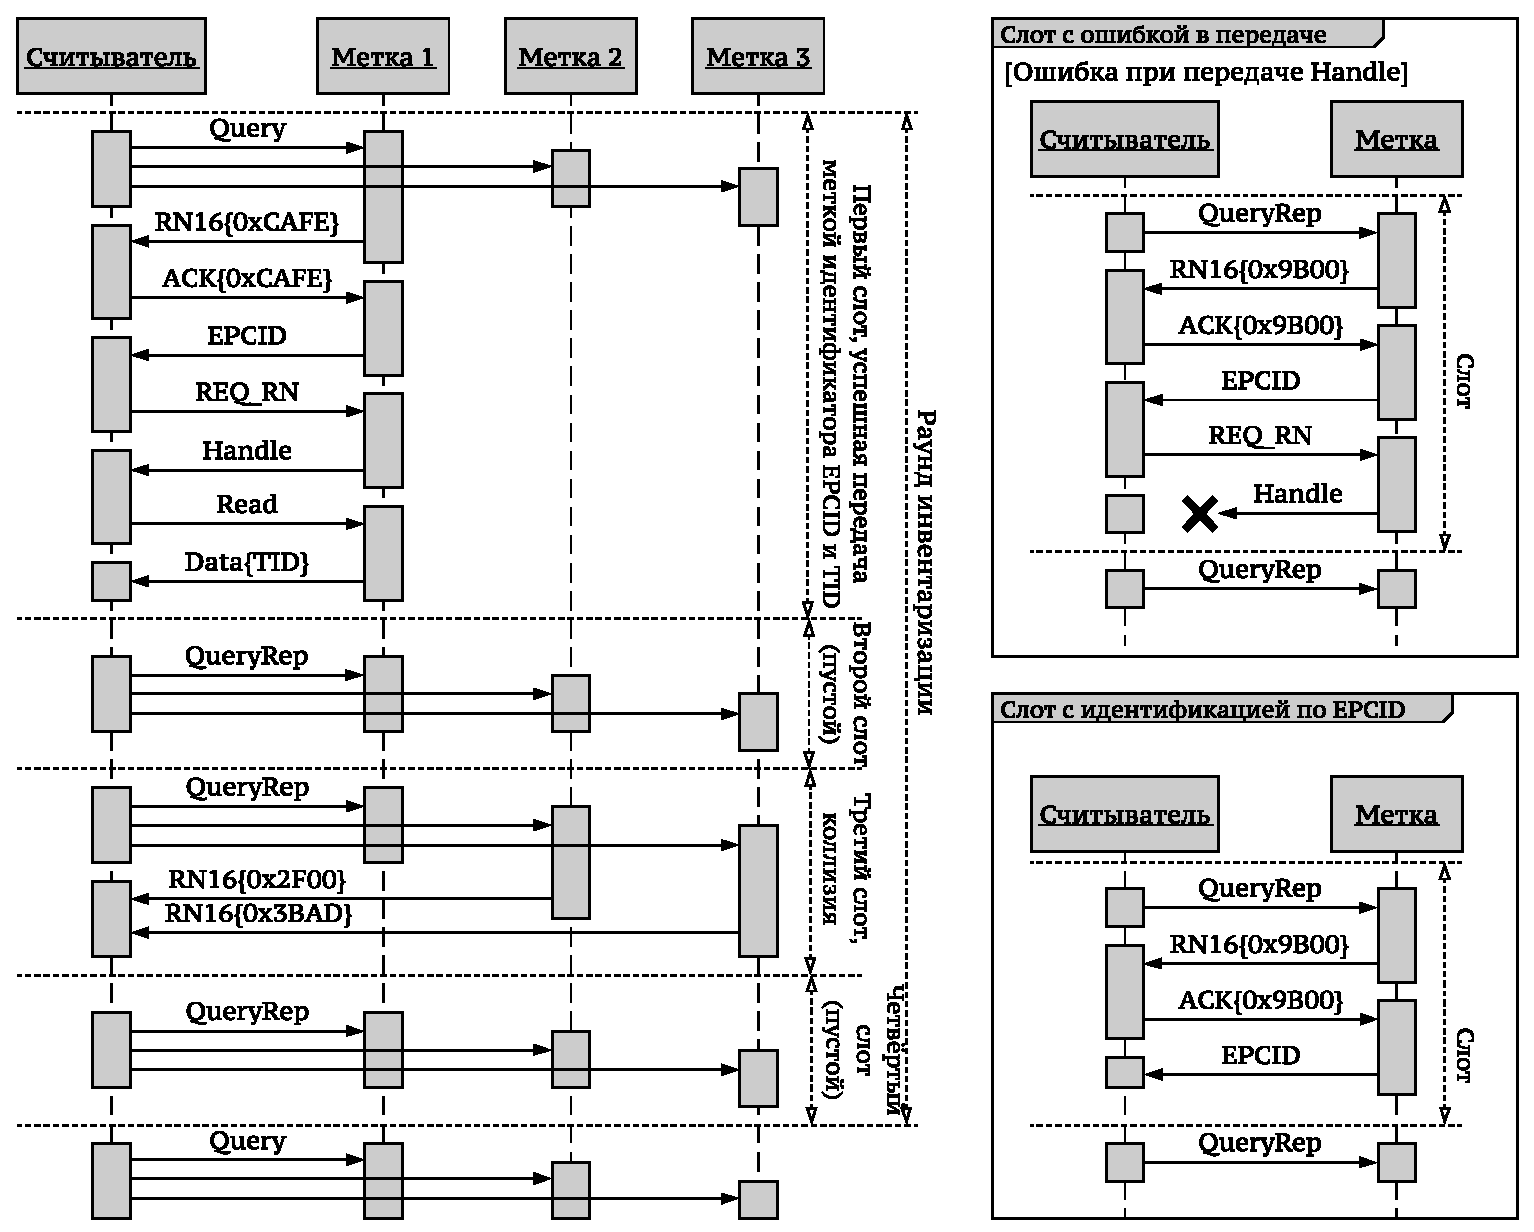
\includegraphics[width=1.0\textwidth]{chapter3/ch3_inventory_round}
  }
  \legend{Справа вверху "--- пример слота, в котором произошла ошибка в передаче ответа Handle. Справа внизу "--- пример слота, в котором метка успешно передает идентификатор, если идентификация происходит только по EPCID.}
  \caption[Пример раунда опроса при идентификации по EPCID и TID.]{Пример раунда инвентаризации с $Q=2$ и числом слотов $N_s=2^Q=4$ в случае идентификации метки по EPCID и TID. }
  \label{fig:ch3_inventory_round}
\end{figure}

Пример раунда инвентаризации показан на рис.~\ref{fig:ch3_inventory_round}. В этом примере предполагается, что параметр $Q = 2$, то есть число слотов $N_s = 2^Q = 4$, и в раунде участвуют три метки. Первая метка выбрала для передачи первый слот, а вторая и третья -- третий. Идентификация метки происходит по комбинации EPCID и TID, поэтому в первом слоте считыватель после получения EPCID запрашивает случайное слово RN16 командой Req\_RN и использует его для контроля доставки в команде Read. В ответ на последнюю метка передает содержимое своего банка памяти TID. Если бы идентификация происходила только по EPCID, то первый слот был бы проще, обмен сообщениями выглядел бы как на правом нижнем фрагменте. Справа вверху показан пример слота, в котором произошла ошибка в передаче одного из ответов. Так как модельный считыватель не передает команды повторно, слот на этом завершается, метка остается неидентифицированной.

Ошибка может произойти при передаче любого из ответов. Учитывая то, что BER постоянен и равен $\beta$, вероятность успешной передачи ответа $\text{msg}$ можно найти как:

\begin{equation}\label{eq:ch3_response_err}
	P_\text{rx}\{\text{msg}\} = (1 - \beta)^{|\text{msg}|},
\end{equation}
где $|\text{msg}|$ -- длина ответа $\text{msg}$ в битах.

В дальнейшем потребуется оценивать число меток, участвующих в очередном раунде. Введём следующее определение.

\begin{defn}
	Назовем метку \textit{активной}, если она находится в области чтения, и ее значение флага сессии совпадает с передаваемым считывателем в поле Target команды Query. Значение этого поля будем называть \textit{флагом опроса}.
\end{defn}
\begin{rem}
	Следует подчеркнуть, что все модельные метки являются пассивными в техническом смысле слова, то есть они работают только в поле действия считывателя и не содержат автономного источника питания. Данное определение активности "--- исключительно логическое. Оно было выбрано, так как наиболее точно и лаконично описывает состояние метки.
\end{rem}

Пусть в начале раунда в системе присутствует $n$ активных меток. Обозначим $\mu_0(n)$ "--- случайное число пустых слотов в этом раунде, $\mu_1(n)$ "--- число слотов с ответом единственной метки без коллизий и $\mu_2(n)$ "--- число слотов с коллизиями. Для дальнейших расчетов нам потребуются распределения вероятностей случайных величин $\mu_0(n)$ и $\mu_1(n)$. Распределение $\mu_0(n)$ определяется следующим образом:

\begin{equation}\label{eq:ch3_empty_slots}
	\mathbb{P}\{\mu_0(n) = z\} = \frac{1}{N_s^n} C_{N_s}^z {n\brace N_s-z} (N_s - z)!,
\end{equation}
где ${ n\brace N_s-z }$ "--- число Стирлинга 2-го рода, то есть число способов разбиения $n$ меток по $N_s - z$ непустым подмножествам.

Вероятность события $\{ \mu_1(n) = m \}$, то есть того, что ровно $m$ из $n$ меток выбрали уникальные слоты и ответят считывателю без коллизий, будем обозначать как $\overline{P}_n(m) = \mathbb{P}\{ \mu_1(n) = m \}$, и будем вычислять с помощью формулы, приведенной в работе \cite{Vales-Alonso2011}:

\begin{equation}\label{eq:ch3_nocol_pnm}
	\overline{P}_n(m) = \mathbb{P}\{ \mu_1(n) = m \} = \frac{N_s! n!}{m! N_s^n} \sum\limits_{z=0}^{n-m}
		\frac{(-1)^z (N_s - m - z)^{(n - m - z)}}{(n - m - z)! z! (N_s - m - z)!}
\end{equation}

Сделаем два замечания относительно формул \eqref{eq:ch3_empty_slots} и \eqref{eq:ch3_nocol_pnm}. Во-первых, в \eqref{eq:ch3_nocol_pnm} предполагается, что число активных меток $n$ не превосходит числа слотов $N_s$. Во-вторых, на практике обе формулы неудобно применять из-за очень больших чисел в числителях и знаменателях уже при $N_s > 8$, то есть $Q = \log_2 N_s > 3$. Частично эту проблему удается решить группировкой множителей, но не во всех случаях, поэтому при численных расчетах для вычисления обеих вероятностей будем пользоваться методом Монте-Карло.

\begin{prop}\label{prop:ch3_pnm}
	Если в раунде инвентаризации участвует $n > 0$ меток, $P_\text{rx}\{\text{RN16}\}$ -- вероятность успешной передачи ответа RN16, а $\overline{P}_n(k)$ -- вероятность того, что ровно $k \leqslant n$ меток выбрали такие слоты, которые не выбрали другие метки, то вероятность того, что ровно $m \leqslant n$ меток изменят после раунда хранимое значение флага определяется следующим выражением:
	\begin{equation}\label{eq:ch3_pnm}
		P_n(m) = \sum\limits_{i=m}^{n}\overline{P}_n(i) C_i^mx \left(P_\text{rx}\{\text{RN16}\}\right)^m
			\left(1 - P_\text{rx}\{\text{RN16}\}\right)^{i - m},\; m \leqslant n
	\end{equation}
\end{prop}
\begin{proof}
	Метка передает идентификатор, если ей пришла команда ACK со случайным словом, совпадающим с переданным ранее меткой в ответе RN16. Согласно сделанным предположениям, это происходит, когда метка передает сообщение RN16 единственной в слоте, и сообщение доставляется без ошибок\footnote{Если бы использовалась более точная модель интерференции, получение ответа было бы возможно также, например, если сигнал от другой метки был в том же слоте, но очень ослабленный.}. Тогда событие $X$:

	$$
	X = \text{<<ровно $m$ из $n$ меток передали идентификаторы>>}
	$$
	можно представить в виде суммы непересекающихся событий $X = \sum\limits_{i=m}^n Y_i$, где:
	$$
	\begin{aligned}
	Y_i = &\text{<<ровно $i$ из $n$ меток передали RN16 без коллизий,}\\
		  &\text{и ровно $m$ из $i$ из них было принято без ошибок>>}.
	\end{aligned}
	$$

	По формуле полной вероятности, учитывая независимость выбора слотов метками и возникновения ошибок в передаче их ответов, а также независимость возникновения ошибок в каждом переданном метками бите, получаем цепочку равенств, доказывающих утверждение:

	\begin{align*}
		P_n(m) &= \mathbb{P}\{X\} = \sum\limits_{i=m}^{n} \mathbb{P}\{Y_i\}\\
		&\begin{aligned}= \sum\limits_{i=m}^{n}(
			&\mathbb{P}\{\text{ровно $i$ из $n$ меток выбрали свободные слоты}\} \times\\
			& \mathbb{P}\{\text{ровно $m$ из $i$ меток успешно передали RN16}\})
			\end{aligned}\\
		&=\sum\limits_{i=m}^{n} \overline{P}_n(i) \times \left(C_i^m(P_\text{rx}\{\text{RN16}\})^m
			(1 - P_\text{rx}\{\text{RN16}\})^{i - m}\right)
	\end{align*}

\end{proof}

Для того, чтобы удостовериться, что $P_n(m)$ корректно описывает вероятность, докажем, что $\sum\limits_{m = 0}^n P_n(m) = \sum\limits_{i=0}^n \overline{P}_n(i) = 1$ (справедливость последнего равенства утверждается в работе \cite{Vales-Alonso2011}). Действительно,
$$
\begin{aligned}
	\sum\limits_{m=0}^n P_n(m) &=
		\sum\limits_{m=0}^n \sum\limits_{i=m}^n \overline{P}_n(i) C_i^m
			P_\text{rx}\{\text{RN16}\}^m (1 - P_\text{rx}\{\text{RN16}\})^{i-m}\\
	&= \sum\limits_{i=0}^n \sum\limits_{m=0}^i \overline{P}_n(i) C_i^m
			P_\text{rx}\{\text{RN16}\}^m (1 - P_\text{rx}\{\text{RN16}\})^{i-m}\\
	&= \sum\limits_{i=0}^n \overline{P}_n(i) \sum\limits_{m=0}^i C_i^m
			P_\text{rx}\{\text{RN16}\}^m (1 - P_\text{rx}\{\text{RN16}\})^{i-m}\\
	&= \sum\limits_{i=0}^n \overline{P}_n(i) \left( P_\text{rx}\{\text{RN16}\} + (1 - P_\text{rx}\{\text{RN16}\}) \right)^i\\
	&= \sum\limits_{i=0}^n \overline{P}_n(i)
\end{aligned}
$$

Вероятность успешной идентификации зависит от того, что используется в качестве идентификатора: EPCID или комбинация TID и EPCID. Условную вероятность успешной идентификации метки при условии отсутствия коллизии и ошибки в передаче RN16 будем обозначать как $p_{\text{id}}$:

\begin{equation}\label{eq:ch3_p_id}
	p_{\text{id}} = \begin{cases}
		P_{\text{rx}}\{\text{EPCID}\}, &\text{только EPCID}\\
		P_{\text{rx}}\{\text{EPCID}\}P_{\text{rx}}\{\text{Handle}\}P_{\text{rx}}\{\text{TID}\},&\text{EPCID и TID}
	\end{cases}
\end{equation}

Для вычисления оценки средней длительности раунда, воспользуемся приближенной схемой расчёта в допущении о независимости определения типов слотов. Будем считать, что каждый слот может принадлежать одному из трех типов: пустой слот (без ответа метки), слот с коллизией (ошибка при передаче RN16) и слот с ответом без коллизии. Обозначим через $t_0$ длительность пустого слота, $t_1^{\text{(epc)}}$ и $t_1^{\text{(tid)}}$  "--- средние длительности слотов с ответом без коллизий при идентификации по EPCID или по TID соответственно, а через $t_2$ "--- длительность слота с коллизией. Эти длительности могут быть вычислены следующим образом:

\begin{equation}\label{eq:ch3_slot_durations}
	\begin{aligned}
		t_0 =\;& T_\text{QRep} + T_1 + T_3\\
		t_1^{\text{(epc)}} =\;& T_\text{QRep} + (T_1 + T_2) +
			T_\text{RN16} + P_{rx}\{\text{RN16}\} \times \\
			&\left( T_\text{ACK} + (T_1 + T_2) + T_\text{EPCID} \right)\\
		t_1^{\text{(tid)}} =\;& T_\text{QRep} + (T_1 + T_2) +
				T_\text{RN16} + P_{rx}\{\text{RN16}\} \times \\
			&( T_\text{ACK} + (T_1 + T_2) + T_\text{EPCID} + P_{rx}\{\text{EPCID}\} \times \\
			&\quad (T_\text{Req\_RN} + (T_1 + T_2) + T_\text{Handle} 	+ P_{rx}\{\text{Handle}\} \times \\
			&\quad\quad(T_\text{Read} +(T_1 + T_2) + T_\text{TID})))\\
		t_1 =\;& \begin{cases}
			t_1^{\text{(epc)}}, &\text{только \text{EPCID}}\\
			t_1^{\text{(tid)}}, &\text{\text{EPCID} и \text{TID}}
 		\end{cases}\\
 		t_2 =\;& T_\text{QRep} + (T_1 + T_2) + T_\text{RN16}
	\end{aligned}
\end{equation}

Согласно допущению, вероятности слотов определяются независимо. Обозначим $p_0(n)$, $p_1(n)$ и $p_2(n)$ веротности того, что произвольный слот пуст, содержит ответ ровно одной метки или коллизию, соответственно. Эти вероятности можно вычислить, используя \eqref{eq:ch3_empty_slots} и \eqref{eq:ch3_nocol_pnm}:

\begin{equation}\label{eq:ch3_slot_probs}
	\begin{aligned}
		p_0(n) =\;& \frac{1}{N_s} \mathbb{E} \mu_0 = \frac{1}{N_s} \sum\limits_{i=0}^{N_s} i \mathbb{P}\{\mu_0 = i\}\\
		p_1(n) =\;& \frac{1}{N_s} \mathbb{E} \mu_1 = \frac{1}{N_s} \sum\limits_{i=0}^{N_s} i \mathbb{P}\{\mu_1 = i\}\\
		p_2(n) =\;& 1 - p_0(n) - p_1(n)
	\end{aligned}
\end{equation}

С помощью соотношений \eqref{eq:ch3_slot_durations} и \eqref{eq:ch3_slot_probs} длительность раунда $\tau(n)$ можно определить как сумму математического ожидания длительности слота и, если после раунда сбрасывается питание, длительности этого сброса:

\begin{equation}\label{eq:ch3_round_duration_of_n}
	\tau_r(n) = N_s \sum\limits_{i=0}^{2}p_i(n)t_i +
		(T_\text{Query} - T_\text{QRep}) +
		e_r T_\downarrow,
\end{equation}
где $n$ "--- число меток, участвующих в раунде, $e_r$ "--- индикатор сброса питания после опроса, а $T_\downarrow$ "--- длительность сброса. Слагаемое $(T_\text{Query} - T_\text{QRep})$ необходимо, так как при расчете длин слотов $t_i$ предполагалось, что каждый слот начинается с команды QRep, хотя первый слот начинается с более длинной команды Query.

Хотя в действительности распределения величин $\mu_0$, $\mu_1$ и $\mu_2$ не являются независимыми, приведенный способ расчета очень простой и позволяет получить достаточно точную оценку длительности раундов. На рис.~\ref{fig:ch3_round_durations_validation} показан расчет с помощью описанной аналитической модели и метода Монте-Карло при различных значениях BER и числе участвующих в опросе меток от 0 до 20 (остальные параметры были фиксированы, число слотов $N_s = 2^Q = 16$). Можно видеть, что допущение о независимости определения типа слота оказывает минимальное влияние на точность оценки.

\begin{figure}[htb]
	\centerfloat{
		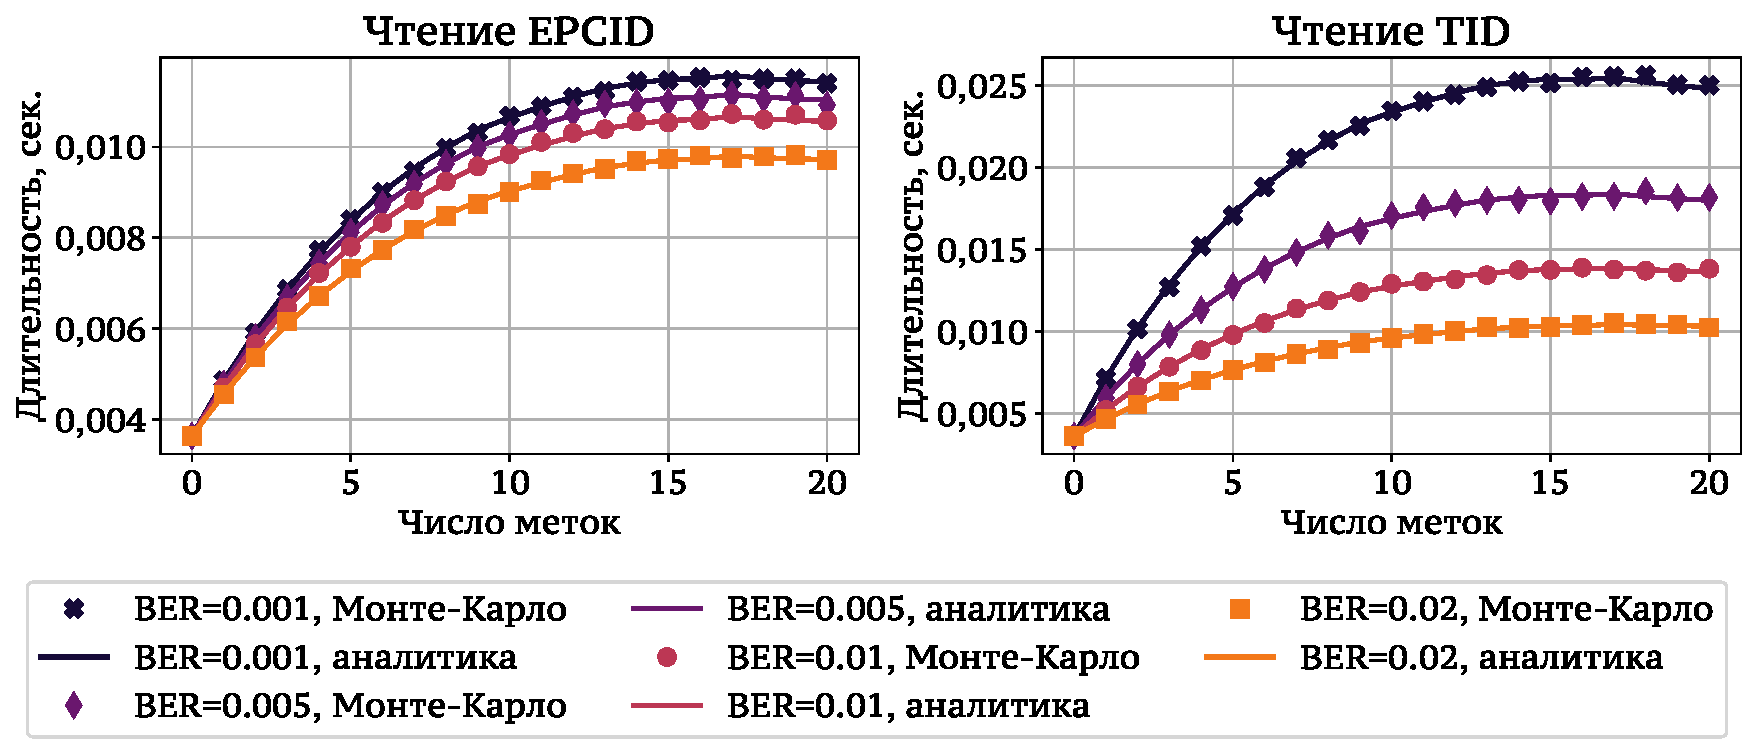
\includegraphics[width=1.0\textwidth]{chapter3/ch3_round_durations_validation.pdf}
  }
  \caption[Валидация модели расчета средрней длительности раундов.]{Сравнение результатов расчета средней длительности раундов с помощью аналитической модели и метода Монте-Карло.}
  \label{fig:ch3_round_durations_validation}
\end{figure}


Если известно распределение вероятностей числа активных меток $\bm{\pi} \in \mathbb{R}^{\overline{N}+1}$, где $\pi_n$ "--- вероятность того, что в системе ровно $n$ активных меток, $n \in [0, \overline{N}]$, то среднюю длину раунда можно опередлить как математическое ожидание $\tau_r = \mathbb{E} \tau_r(n)$:

\begin{equation}\label{eq:ch3_round_duration_avg}
	\tau_r = \sum\limits_{n=0}^{\overline{N}} \pi_n \tau_r(n)
\end{equation}

Пользуясь выражениями для длительностей слотов $t_1, t_2$ и $t_3$, можно найти оценку максимальной длительности раунда $\tau_{max}$:

\begin{equation}\label{eq:ch3_max_round_duration}
	\tau_{max} = \begin{cases}
 		\overline{N} t_1 + (N_s - \overline{N}) t_0, &\overline{N} \leqslant N_s\\
 		(N_s - 1) t_1 + t_2, &\overline{N} > N_s.
 	\end{cases}
\end{equation}
Справедливость этого выражения следует из того, что $t_0 < t_2 < t_1$ (значение $T_3$ заведомо не превышает $T_\text{RN16}$): если слотов больше, чем меток, то максимум достигается, когда все метки успешно передают свои идентификаторы. Если же слотов меньше, то в самом длинном раунде все слоты кроме одного будут содержать успешные передачи, а в одном слоте произвойдет коллизия оставшихся $\overline{N} - (N_s - 1)$ меток.



%%%%%%%%%%%%%%%%%%%%%%%%%%%%%%%%%%%%%%%%%%%%%%%%%%%%%%%%%%%%%%%%%%%%%%%%%%%%%%%%
\section{Вычисление оценки длительностей раундов}\label{sec:ch3_round_durations}
%%%%%%%%%%%%%%%%%%%%%%%%%%%%%%%%%%%%%%%%%%%%%%%%%%%%%%%%%%%%%%%%%%%%%%%%%%%%%%%%

%%% --------------------------------------------
\subsection{Размеченные сценарии и элементарные операции}
%%% --------------------------------------------
Пусть в некоторый момент времени в системе находится $N$ меток, $0 \leqslant N \leqslant \overline{N}$, и пусть $n$ из них активны, то есть готовы принять участие в раунде, в котором опрос просходит по флагу $X \in \{A, B\}$, $0 \leqslant n \leqslant N$.

Число $n$ может измениться по трем причинам (см. рис.~\ref{fig:ch3_operations}). Во-первых, если флаг опроса $X$ после очередного раунда инвентаризации не изменяется, и $n' \leqslant n$ меток в этом раунде передали свои EPCID, то эти метки инвертировали свои флаги и в следующем раунде не будут принимать участие, то есть активными будут $n - n'$ меток. Если же после раунда считыватель инвертирует флаг опроса $X$, то число активных меток будет $N - (n - n')$. Во-вторых, само число $N$ может измениться, если какая-либо метка покинула систему, или, наоборот, вошла в нее. Это изменение может затронуть число активных меток $n$, если систему покинула активная метка (в этом случае $n$ уменьшается на единицу), или если метка поступила в систему, и текущий флаг опроса равен $A$ (значение $n$ увеличивается на единицу). Наконец, в-третьих, считыватель может сбросить питание, после чего все метки будут хранить значение флага, равное $A$. Если считыватель продолжит опрос с флагом $X = A$, то активными будут все $n = N$ меток, а если с флагом $B$, то активных меток точно не будет, $n = 0$.

\begin{figure}[htb]
	\centerfloat{
    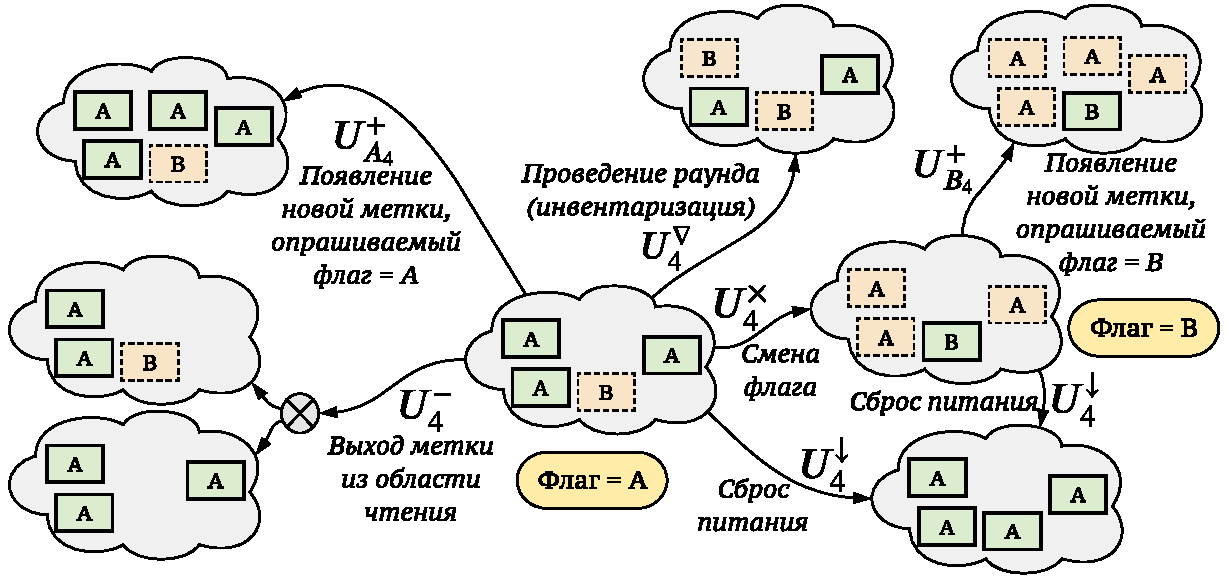
\includegraphics[width=1.0\textwidth]{chapter3/ch3_operations}
  }
  \caption{Операции над системой.}
  \label{fig:ch3_operations}
\end{figure}

Таким образом, изменение числа активных меток происходит в результате пяти действий, которые в дальнейшем будем называть \textit{элементарными операциями}: проведения раунда инвентаризации ($U_N^\nabla$), изменения флага опроса ($U_N^\times$), сброса питания ($U_N^\downarrow$), добавления метки в систему ($U_N^+$) или выхода метки ($U_N^-$). Как будет показано далее, с помощью композиции элементарных операций можно описать, как изменяется распределение числа активных меток после каждого раунда. Однако первый вопрос "--- как по известному сценарию работы считывателя определить, какие элементарные операции нужно выполнять.

В начале главы было введено понятие сценария (см. определение~\ref{def:ch3_reader_scenario}) как последовательности $\bm{\alpha} = \alpha_1 \alpha_2 \dots \alpha_R$, где $\alpha_r = (X_r, e_r) \equiv X_r^{e_r}$ "--- спецификация раунда. По заданному сценарию можно описать операцию, которую считыватель должен провести над метками. Например, если $\bm{\alpha} = \alpha_1 \alpha_2 \alpha_3 \alpha_4 = A^0 B^1 A^0 A^1$, то в первом раунде нужно провести опрос ($U_N^\nabla$) и инвертировать флаг опроса с $A$ на $B$ ($U_N^\times$), во втором раунде "--- провести опрос и сбросить питание ($U_N^\downarrow$), в третьем раунде просто провести опрос, а в четвертом "--- провести опрос и сбросить питание.

В сценарии содержится только информация о работе считывателя, однако нет данных о том, когда метки появляются и выходят из системы. Обозначим число меток в области чтения в $r$-м раунде как $N_r$, а число меток, покидающих и поступающих в область чтения за время $r$-го раунда как, соответственно, $\Delta_r^-$ и $\Delta_r^+$.  Предположим, что удалось установить, сколько меток было в области чтения в начале первого раунда $N_1$, а также все значения $\{\Delta_r^-\}_{r=1}^R$ и $\{\Delta_r^+\}_{r=1}^R$. Отметим, что для раунда $r > 1$ число меток можно вычислить как $N_r = N_{r-1} - \Delta_{r-1}^- + \Delta_{r-1}^+$.  Введем следующее определение, объединяющее сценарий $\bm{\alpha}$ и оценки $\{ N_r \}$, $\{ \Delta_r^- \}$ и $\{ \Delta_r^+ \}$.

\begin{defn}\label{ref:ch3_marked_scenario}
  Будем называть \textit{размеченным сценарием} последовательность символов $\widetilde{\bm{\alpha}} = \widetilde{\alpha}_1 \widetilde{\alpha}_2 \dots \widetilde{\alpha}_R$, каждый из которых имеет вид пятерки $\alpha_r = (X_r, e_r ; N_r, \Delta^-_r, \Delta^+_r)$. Символы $\alpha_r$ будем называть \textit{размеченными спецификациями раундов}. В дальнейшем будем использовать нотацию $[\prescript{N_r}{\Delta_r^-} X_{\Delta_r^+}^{e_r}]$, причем для сокращения записи иногда не будем указывать $\Delta_r^-$, $\Delta_r^+$ и $e_r$, если они равны нулю.
\end{defn}


Возвращаясь к предыдущему примеру, если сценарий $\bm{\alpha} = A^0 B^1 A^0 A^1$, $N_1 = 5$, $\{ \Delta_r^+ \} = \{ 0, 1, 0, 1 \}$ и $\{ \Delta_r^- \} = \{ 1, 0, 0, 1 \}$, то $\{ N_r \} = \{ 5, 4, 5, 5 \}$ и
$$
\begin{aligned}
	\widetilde{\bm{\alpha}} &= \left( (A, 0; 5, 1, 0),\,
	(B, 1; 4, 0, 1),\,
	(A, 0; 5, 0, 0),\,
	(A, 1; 5, 1, 1)\right) =\\
	&= [\prescript{5}{1} A^{0}_{0}] [\prescript{4}{0} B^{1}_{1}] [\prescript{5}{0} A^{0}_{0}] [\prescript{5}{1} A^{1}_{1}]
		= [\prescript{5}{1}A] [B^{1}_{1}] [\prescript{5}{}A] [\prescript{5}{1} A^{1}_{1}]
\end{aligned}
$$
Для такого размеченного сценария уже можно полностью описать все действия над системой: в первом раунде после опроса ($U_5^\nabla$) нужно инвертировать флаг ($U_5^\times$) и удалить метку ($U_{B,5}^+$), во втором раунде "--- провести опрос ($U_4^\nabla$), сбросить питание ($U_4^\downarrow$) и добавить одну метку ($U_{A,4}^+$), в третьем "--- только провести опрос ($U_5^\nabla$), а в четвертом "--- провести опрос ($U_5^\nabla$), сбросить питание ($U_3^\downarrow$), удалить одну метку ($U_5^-$) и затем добавить еще одну метку ($U_{A,4}^+$). Отметим, что пример последнего раунда показывает, почему недостаточно знать число меток в каждом раунде, а важно также знать, сколько меток поступает и покидает область чтения.

Для построения размеченного сценария нужно найти число меток перед первым раундом, а также определить, сколько меток поступает и покидает систему в каждом раунде. Пусть модельное время начинается в момент $T_0$. Обозначим последовательность моментов начала раундов опросов как $\{ t_r \}_{r=1}^\infty$. Тогда $\Delta_r^+ = |\{ a_i :\: t_r \leqslant a_i < t_{r+1} \}|$ и $\Delta_r^- = |\{ a_i:\: t_r \leqslant a_i + T_L < t_{r+1} \}|$, а $N_1 = N(T_0)$. Таким образом, для нахождения $\Delta_r^-$ и $\Delta_r^+$ нужно знать, когда начинается каждый раунд, а для этого нужно вычислить оценки длительностей каждого раунда $\{ \tau_r \}$. Длительности раундов опроса $\{ \tau_r \}$ вычисляются с помощью выражений \eqref{eq:ch3_round_duration_of_n} и \eqref{eq:ch3_round_duration_avg}, но для их использования нужно знать распределение вероятностей числа меток $n$, принимающих участие в каждом раунде.

Прежде, чем перейти к решению вопроса о нахождении оценок длительностей раундов, отметим, что значение $N_r$ можно вычислить, как $N_r = N(T_0 + \tau_1 + \tau_2 + \dots + \tau_{r-1}).$ Величина $T_0$ может быть произвольной, но желательно устанавливать ее достаточно большой, чтобы избежать погрешности из-за краевых эффектов.


%%% --------------------------------------------
\subsection{Матрицы элементарных операций}\label{subsec:ch3_bg_elem_op_matrices}
%%% --------------------------------------------
Как отмечалось ранее, число активных меток является случайной величиной, так как в общем случае вероятность того, что в течение раунда инвентаризации ровно $n - n'$ меток передадут свои идентификаторы, меньше единицы. Рассмотрим случайный процесс $\{ \eta_r \in [0, \overline{N}] \}_{r=1}^\infty$, моделирующий число активных меток в системе. Время в этом процессе дискретно и увеличивается на единицу после выполнения операции. В дальнейшем, в качестве такой операции будет выступать выполнение раунда и всех действий, определенных спецификацией. Однако, в этом разделе, прежде чем ввести определение операции, моделирующей весь раунд, для удобства будем считать, что $r$ меняется после каждой \textit{элементарной} операции.

Пусть $U$ "--- одна из элементарных операций, число активных меток перед ее выполнения равно $\eta_r = n$, а после "--- $\eta_{r+1} = n'$, $n,n' \in [0,\overline{N}]$. В силу сделанных ранее допущений, в частности "--- о постоянстве BER во всей области чтения, каждую элементарную операцию будем задавать распределением вероятностей $\mathbb{P}\{\eta_{r+1} = n' | \eta_r = n\}$. Переходные вероятности операции $U$ можно задать в виде матрицы порядка $\overline{N} + 1$. Для удобства будем считать, что нумерация строк и столбцов в матрицах $U$ и элементов вектора $\bm{\pi}$ начинается с нуля, чтобы номера строк и столбцов в точности соответствовали числу активных меток; тогда $\{ U \}_{ij} = \mathbb{P}\{ \eta_{r+1} = j\; |\; \eta_{r} = i \}$. Рассмотрим переходные матрицы каждой из элементарных операций (см. рис.~\ref{fig:ch3_bg_trans}).

\begin{figure}[htb]
	\centerfloat{
    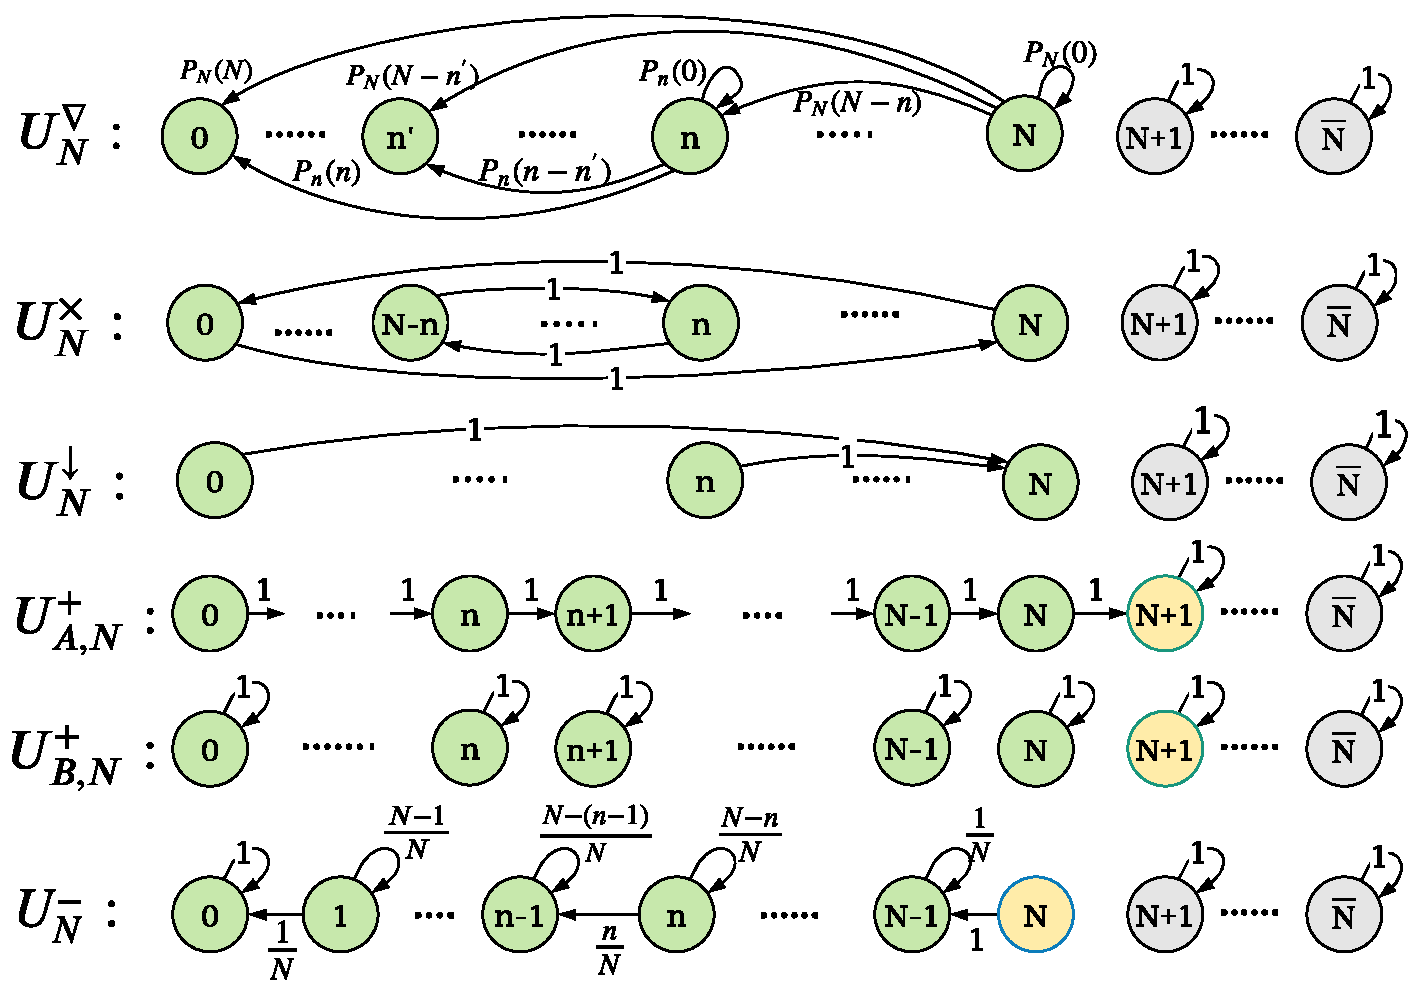
\includegraphics[width=0.9\textwidth]{chapter3/ch3_bg_trans}
  }
  \caption{Изменение числа активных меток при выполнении элементарных операций.}
  \label{fig:ch3_bg_trans}
\end{figure}

Применение операции опроса меток приводит к том, что часть меток передают (возможно, успешно) свои EPCID и инвертируют флаг. Непосредственно после этой операции флаг не меняется, питание не отключается, а метки не покидают и не поступают в область чтения. Вероятность того, что после опроса ровно $n'$ из $n$ меток будут активны, равна $P_n(n - n')$ (см. выражение~\eqref{eq:ch3_pnm}), а матрица $U_N^\nabla$ задается так:

\begin{equation}\label{eq:ch3_bg_inventory}
	\{ U_N^\nabla \}_{ij} = \begin{cases}
		P_i(i - j), & 0 \leqslant j \leqslant i \leqslant N\\
		1,          & N < i = j \leqslant \overline{N}\\
		0,          & \text{в остальных случаях.}
 	\end{cases}
\end{equation}

В результате инвертирования флага опроса неактивные метки становятся активными и наоборот, и число активных меток становится равным $N - n$:

\begin{equation}\label{eq:ch3_bg_switch}
	\{ U_N^\times \}_{ij} = \begin{cases}
 		1, & 0 \leqslant i \leqslant N,\; j = N - i\\
 		1, & N < i = j \leqslant \overline{N}\\
 		0, & \text{в остальных случаях.}
 	\end{cases}
\end{equation}

Сброс питания приводит к тому, что у всех меток в области чтения хранимое значение флага становится равным $A$. Так как после этого опрашивать метки по флагу $B$ не имеет практического смысла, будем считать, что флаг опроса также становится равным $A$, то есть все метки "--- активны:

\begin{equation}\label{eq:ch3_bg_power_off}
	\{ U_N^\downarrow \}_{ij} = \begin{cases}
 		1, & 0 \leqslant i \leqslant N,\; j = N\\
 		1, & N < i = j \leqslant \overline{N}\\
 		0, & \text{в остальных случаях.}
 	\end{cases}
\end{equation}

Выполнение операции добавления метки ведет к тому, что в системе становится на одну метку больше (то есть увеличивается $N$). Изменение числа активных меток зависит от текущего значения флага опроса: если флаг опроса $X = A$, то число активных меток увличивается, а если $X = B$, не изменяется:

\begin{equation}\label{eq:ch3_bg_tag_arrival}
	\begin{aligned}
		\{ U_{A,N}^+ \}_{ij} &= \begin{cases}
			1, & 0 \leqslant i < \overline{N}, \; j = i + 1\\
			1, & N+1 \leqslant i = j \leqslant \overline{N}\\
			0, & \text{в остальных случаях}
	 	\end{cases}\\
		U_{B,N}^+ &= I_{\overline{N}+1},
 	\end{aligned}
\end{equation}
где $I_{\overline{N}+1}$ "--- единичная матрица порядка $\overline{N}+1$.

Наконец, при выходе метки из области чтения число меток $N$ уменьшается. Изменение числа активных меток зависит от того, была ли покинувшая систему метка активной. Здесь необходимо сделать одно замечание. В идеале, нужно учитывать, какая метка находится ближе к области выхода, и смотреть, активна ли она. Однако, это привело бы к серьезному увеличению пространства состояний: вместо одного числа активных меток нужно было бы хранить в состоянии системы положения меток и значения их флагов. Поэтому при определении этой элементарной операции сделаем допущение о том, что покинуть систему может равновероятно любая метка. В этому случае вероятность изменения числа активных меток пропорциональна их числу в системе:

\begin{equation}\label{eq:ch3_bg_tag_departure}
	\{ U_{N}^- \}_{ij} = \begin{cases}
		\frac{i}{N},     & 0 < i \leqslant N,\; j = i - 1\\
		\frac{N - i}{N}, & 0 \leqslant i < N,\; i = j\\
		1,               & N \leqslant i = j \leqslant \overline{N}\\
		0,               & \text{в остальных случаях.}
 	\end{cases}
\end{equation}

Прежде, чем перейти к моделированию раундов инвентаризации, сделаем замечание относительно элементов матриц. Можно видеть, что во всех матрицах справа внизу содержится единичный блок. Вообще говоря, строки при $i > N$ не имеют физического смысла: любая операция вида $U^\bullet_N$ применяется к системе, в которой находится $N$ меток. Было бы логично сделать так, чтобы все матрицы имели порядок $N+1$ ($N+2$ для $U_N^+$), то есть чтобы каждый элемент соответствовал возможному изменению числа активных меток, учитывая, что в системе перед выполнением операции находится ровно $N$ меток. Однако, далее потребуется рассматривать композиции элементарных операций, для чего их матрицы будут перемножаться. Можно видеть, однако, что вероятность попадания в состояние $n > N$ в результате выполнения любой из операций (за исключением $U_N^+$) равна нулю, и любое из состояний $n > N$ является поглощающим.




%%% --------------------------------------------
\subsection{Построение операций по размеченному сценарию}\label{subsec:ch3_bg_op_composition}
%%% --------------------------------------------
Обозначим распределение вероятностей случайной величины $\eta_r$ как $\bm{\pi}^{(r)} \in \mathbb{R}^{\overline{N}+1}$. Здесь $\pi_n^{(r)} = \mathbb{P}\{\eta_r = n \}$ при $n \in [0, N_r]$, и $\pi_n^{(r)} \equiv 0$ при $n > N_r$. Если перед выполнением элементарной операции $U_i$ распределение вероятностей $\eta$ было $\bm{\pi}$, то распределение после ее выполнения будет $\bm{\pi}U_i$, после выполнения $U_{i+1}$ распределение будет $\bm{\pi} U_i U_{i+1}$ и так далее. Действительно, учитывая, что вероятность изменения $\eta_r$ вследствие выполнения операции определяется только текущим значением $\eta_r$ и типом элементарной операции, случайный процесс $\{ \eta_r \}$ будет неоднородным марковским процессом с дискретным временем, матрицы переходов которого есть матрицы операций.

\begin{figure}[htb]
	\centerfloat{
    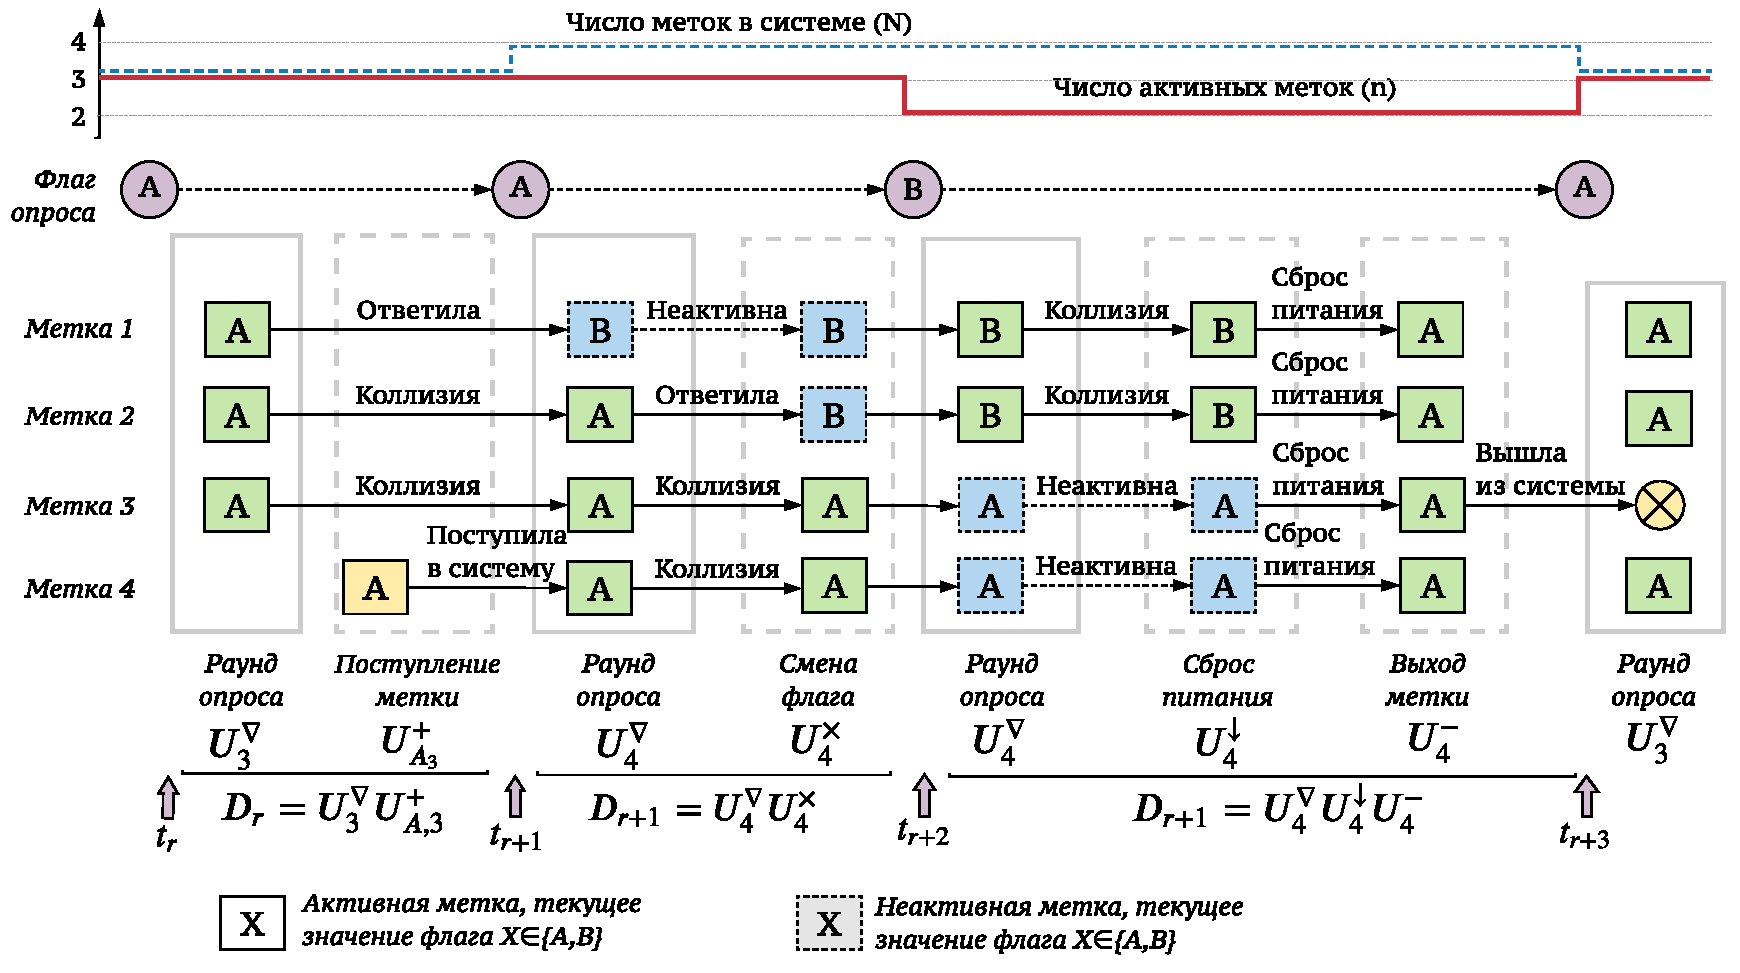
\includegraphics[width=1.0\textwidth]{chapter3/ch3_decomposition}
  }
  \caption{Пример представления раундов в виде операций, и декомпозиция этих операций до элементарных операций.}
  \label{fig:ch3_decomposition}
\end{figure}

Представим весь процесс изменения состояния системы в виде последовательности операций $D_r$, по одной операции на раунд опроса. Каждую операцию $D_r$ можно представить в виде композиции элементарных операций (см. пример~\ref{fig:ch3_decomposition}). Отсюда и далее будем полагать, что время в слуайном процессе $\eta_r$ (число активных меток) меняется на единицу в начале каждого раунда.

Рассмотрим расширенный размеченный сценарий $\widetilde{\bm{\alpha}} = \widetilde{\alpha}_1 \widetilde{\alpha}_2 \dots \widetilde{\alpha}_R$. Пусть $\widetilde{\alpha}_r = (X, N, e, \Delta^-, \Delta^+)$ и $\widetilde{\alpha}_{r+1} = (Y, \bullet, \bullet, \bullet, \bullet)$ (здесь $\bullet$ "--- произвольное значение). Все, что происходит с системой в $r$-м раунде, полностью описывается значениями текущего флага опроса $X$, числом меток $N$, количеством покидающих и поступающих в систему меток $\Delta^-$ и $\Delta^+$, признаком сброса питания после опроса $e$ и значением флага в следущем раунде $Y$.

\begin{figure}[htb]
	\centerfloat{
    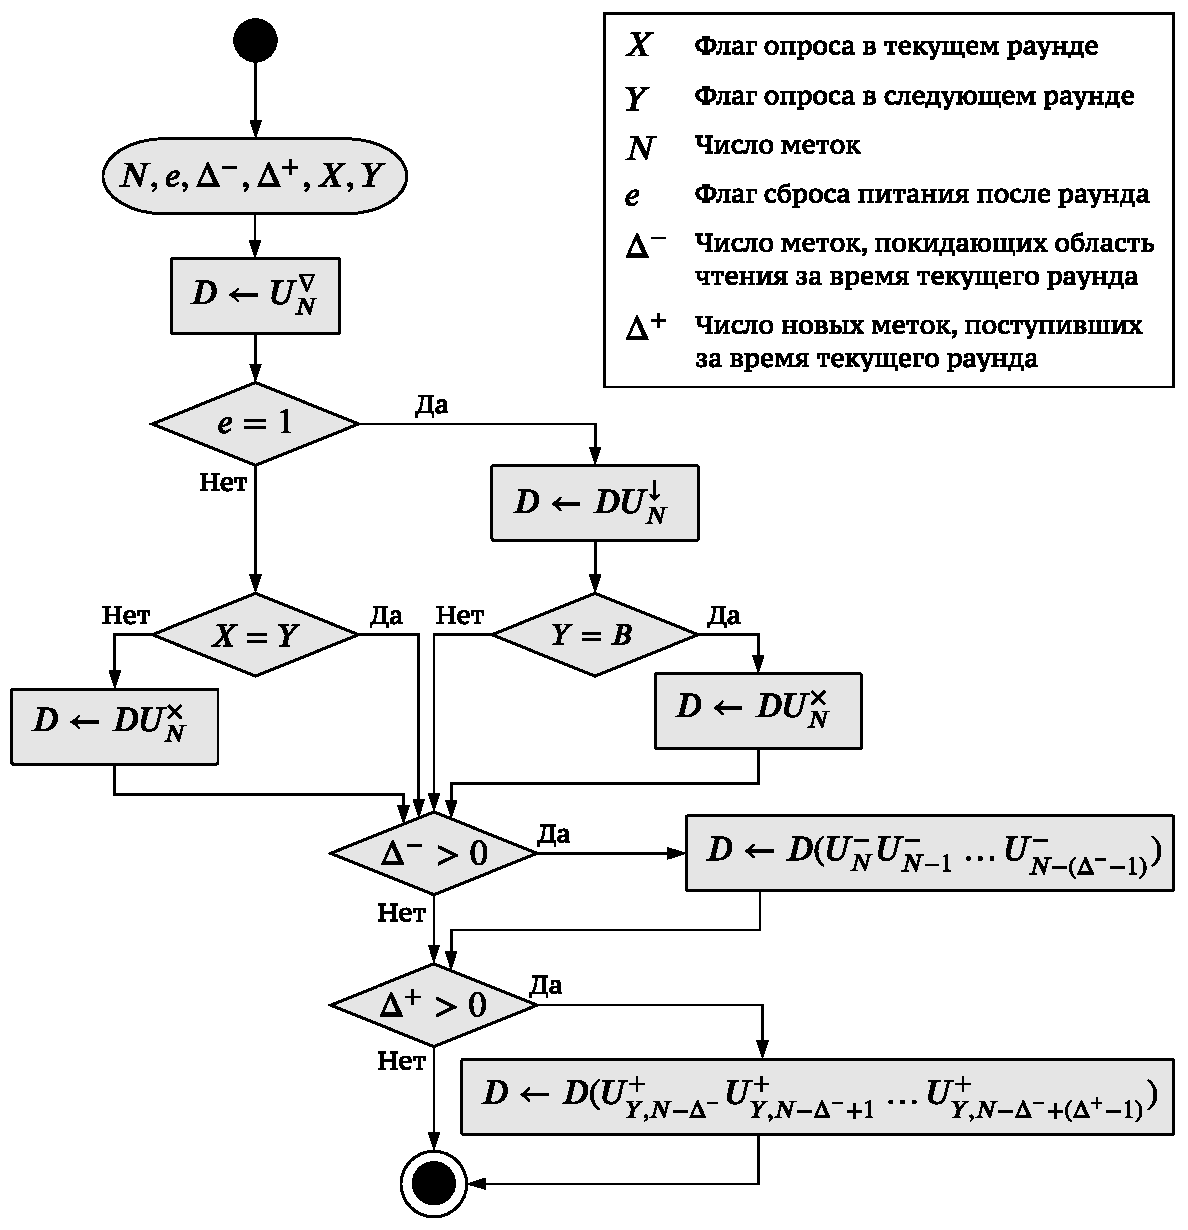
\includegraphics[width=0.8\textwidth]{chapter3/ch3_matrix_composition}
  }
  \caption{Алгоритм построения матрицы перехода $D$.}
  \label{fig:ch3_matrix_composition}
\end{figure}

Алгоритм построения матрицы $D = D_r$ приведен на рис.~\ref{fig:ch3_matrix_composition}. Матрица $D$ представляется в виде произведения матриц элементарных операций $U_i$, причем первым множителем в этом произведении всегда является $U_N^\nabla$, то есть матрица операции инвентаризации меток. Далее, если считыватель выключается, то нужно умножить $D$ на $U^\downarrow_N$ и, если в следующем раунде считыватель опрашивает метки по флагу $Y = B$, умножить на матрицу операции смены флага $U^\times_N$. Если считыватель не выключается, то $D$ нужно умножить на матрицу $U^\times_N$ в том случае, если флаг опроса в следующем раунде инвертируется, то есть $X \neq Y$. Если за время опроса и отключения (если $e = 1$) счиытывателя одна или более меток покинули область чтения, то есть $\Delta^- > 0$, то умножаем $D$ на матрицы $U^-_N, U^-_{N-1}, \dots, U^-_{N-(\Delta^--1)}$ (так как после каждой операции вида $U^-_N$ число меток в области чтения становится меньше на единицу, уменьшается и нижний индекс). Если за время опроса в систему поступили метки, то есть $\Delta^+ > 0$, то аналогично умножаем матрицу $D$ на матрицы операций добавления меток $U^+_{Y,N'}, U^+_{Y,N'+1}, \dots, U^+_{Y,N+(\Delta^+-1)}$, где $N' = N - \Delta^-$.

Отметим, что порядок умножения матриц элементарных операций важен. К примеру, пусть в раунде $r+1$ считыватель ведет опрос по флагу $A$, и с ненулевой вероятностью все метки в конце раунда $r$ хранят флаг $B$, то есть число активных меток равно нулю ($\eta_r = 0$). Пусть также после раунда $r$ одна метка поступает в систему, а другая "--- покидает ее. Новая метка всегда хранит флаг сессии со значением $A$, то есть в данном случае будет активной в раунде $r+1$. Очевидно, что после этого в начале $(r+1)$-го раунда в системе обязательно будет хотя бы одна активная метка. Но если бы операция добавления учитывалась до операции удаления метки, то с вероятностью $1/{(N+1)}$ число активных меток уменьшилось бы до нуля. По тем же причинам, смена флага должна учитываться до добавления меток, но после сброса питания.

Вернемся к примеру расширенного сценария $\widetilde{\bm{\alpha}} = [\prescript{5}{1}A^{0}_{0}] [\prescript{4}{0} B^{1}_{1}] [\prescript{5}{0}A^{0}_{0}] [\prescript{5}{1}A^{1}_{1}]$. Для него представление в виде операций, моделирующих раунды, и декомпозиция до уровня элементарных операций будет выглядеть так:

$$
\begin{aligned}
  \widetilde{\bm{\alpha}} =&
  [\prescript{5}{1}A^{0}_{0}] [\prescript{4}{0}B^{1}_{1}] [\prescript{5}{0}A^{0}_{0}] [\prescript{5}{1}A^{1}_{1}]
  	\Longrightarrow D_1\,, D_2\,, D_3\,, D_4, \text{ где}\\
  &\qquad D_1 = U^\nabla_5 U^\times_5 U^-_5\\
  &\qquad D_2 = U^\nabla_4 U^\downarrow_4 U^+_{A,4}\\
  &\qquad D_3 = U^\nabla_5\\
  &\qquad D_4 = U^\nabla_5 U^\downarrow_5 U^-_5 U^+_{A,4}
\end{aligned}
$$




%%% --------------------------------------------
\subsection{Расчет распределения числа активных меток}
%%% --------------------------------------------
Имея последовательность операций для размеченного сценария, можно рассчитать распределение вероятностей числа активных меток перед началом каждого раунда. Как отмечалось выше, случайный процесс $\eta_r$ "--- неоднородный марковский. Время в этом процесе увличивается на единицу на каждом раунде, а матрицами переходов являются $D_1, D_2, \dots D_R$. Так как после выполнения сценария ситема моделируется опять с начала  размеченного сценария, то после операции $D_R$ будут опять применяться операции $D_1, D_2, \dots D_R$. В общем случае можно записать это так:
$$
	D_r \equiv D_{(r - 1)\, (\textbf{mod } R) + 1}.
$$

Если процесс $\eta_r$ на $r$-м шаге имеет распределение $\bm{\pi}^{(r)}$, то после $r$-го раунда распределение будет $\bm{\pi}^{(r)} D_r$, после $r+1$ шага "--- $\bm{\pi}^{(r)} D_r D_{r+1}$ и так далее. Так как после $R$-й переходной матрицы опять используется $D_1$, то распределение процесса на $(r+R)$-м шаге будет
$$
	\bm{\pi}^{(r+R)} = \bm{\pi}^{(r)} D_r D_{r+1} \dots D_R D_1 \dots D_{r-1}.
$$
Обозначим произведение матриц, стоящих в правой части, как $\widetilde{D}_{r}$, то есть положим
$$
	\widetilde{D}_r = D_r D_{r+1} \dots D_R D_1 \dots D_{r-1}.
$$

Рассмотрим последовательность значений процесса $\{ \eta_r \}$ на шагах $r, r+R, r+2R, \dots$ и обозначим эту последовательность как $\{ \eta_i^{[r]} \}_{i=0}^\infty$, $\eta_i^{[r]} = \eta_{r+Ri}$. Так как процесс $\{ \eta_{i}^{[r]} \}$ является вложенным процессом в марковский процесс $\{ \eta_r \}$, то он и сам является марковским, причем в отличии от $\{ \eta_r \}$ однородным: переходные матрицы между шагами задаются матрицей $\widetilde{D}_r$. Найти его стационарное распределение $\bm{\pi}^{(r)}$ можно из системы линейных уравнений:
$$
	\begin{cases}
		\bm{\pi}^{(r)} &= \bm{\pi}^{(r)} \widetilde{D}_r\\
		1 &= \sum\limits_{n=0}^{\overline{N}} \pi^{(r)}_n
	\end{cases}
$$
Из найденного вектора $\bm{\pi}^{(r)}$ можно найти $\bm{\pi}^{(r+1)} = \bm{\pi}^{(r)} D_r$, $\bm{\pi}^{(r+2)} = \bm{\pi}^{(r+1)} D_{r+1}$ и так далее. Таким образом, рассчитать распределение вероятностей перед каждым раундом $r = 1, 2, \dots, R$ можно, решив следующую систему уравнений:

\begin{equation}\label{eq:ch3_bg_pmf_system}
	\begin{cases}
		\bm{\pi}^{(1)} &= \bm{\pi}^{(1)} \widetilde{D}_1\\
		\bm{\pi}^{(2)} &= \bm{\pi}^{(1)} D_1\\
		\bm{\pi}^{(3)} &= \bm{\pi}^{(2)} D_2\\
		\dots&\\
		\bm{\pi}^{(R)} &= \bm{\pi}^{(R-1)} D_{R-1}\\
		1              &= \sum\limits_{n=0}^{\overline{N}} \pi^{(1)}_n
	\end{cases}
\end{equation}

Используя найденные распределения числа активных меток, с помощью формул \eqref{eq:ch3_round_duration_of_n} и~\eqref{eq:ch3_round_duration_avg} можно вычислить новые оценки длительностей раундов $\tau_r = \mathbb{E} \tau_r(n)$.



%%% --------------------------------------------
\subsection{Итерационный расчет оценок длительностей раундов}\label{subsec:ch3_iterative_algorithm}
%%% --------------------------------------------
В результате расчета $\tau_r$ по найденным распределениям $\{ \bm{\pi}^{(r)} \}_{r=1}^R$ оценки длительностей раундов могут измениться. Если изначально раунды предполагались сликом короткими или длинными, то после того, как будет найдено распределение числа активных меток, их длительности могут соответственно увеличиться или уменьшиться. Так как моменты поступления меток $\{a_i\}$ и закон изменения числа меток $N(t)$ не зависят от длительностей раундов, то может измениться и размеченный сценарий.

Рассмотрим пример. Пусть задан сценарий $\bm{\alpha} = A^0 A^0 A^0 \dots$, в начальный момент в системе две метки и новая метка поступает на 120-й миллисекунде ($a_1 = 120$). Предположим изначально, что первые два раунда имеют длительность 100~миллисекунд (то есть $\tau_1 = \tau_2 = 100$). Тогда размеченный сценарий будет иметь вид $\widetilde{\alpha} = [\prescript{2}{}A] [\prescript{2}{}A_1] [\prescript{3}{}A] \dots$. Если после пересчета выяснится, что раунды имеют длительности $\tau_1 = 150$ и $\tau_2 = 95$, то новый размеченный сценарий будет иметь вид $\widetilde{\alpha}' = [\prescript{2}{}A_1] [\prescript{3}{}A_1] \dots$. Соответственно, изменятся и матрицы переходных вероятностей операций $D_r$, поэтому в итоге могут измениться и оценки $\{ \bm{\pi}^{(r)} \}$, и $\{ \tau_r \}$. Таким образом, может потребоваться многократный пересчет оценок $\tau_r$.

Итерационный алгоритм, позволяющий найти оценки длительностей раундов $\{ \tau_r \}$, принимает на вход сценарий $\bm{\alpha} = \alpha_1 \alpha_2 \dots \alpha_R$, закон изменения числа меток $N(t)$, максимально допустимую ошибку $\epsilon > 0$ и максимальное число итераций $\overline{K}$. Алгоритм выполняет следующие действия (см. рис.~\ref{fig:ch3_iterative_algorithm}).

\begin{figure}[htb]
	\centerfloat{
    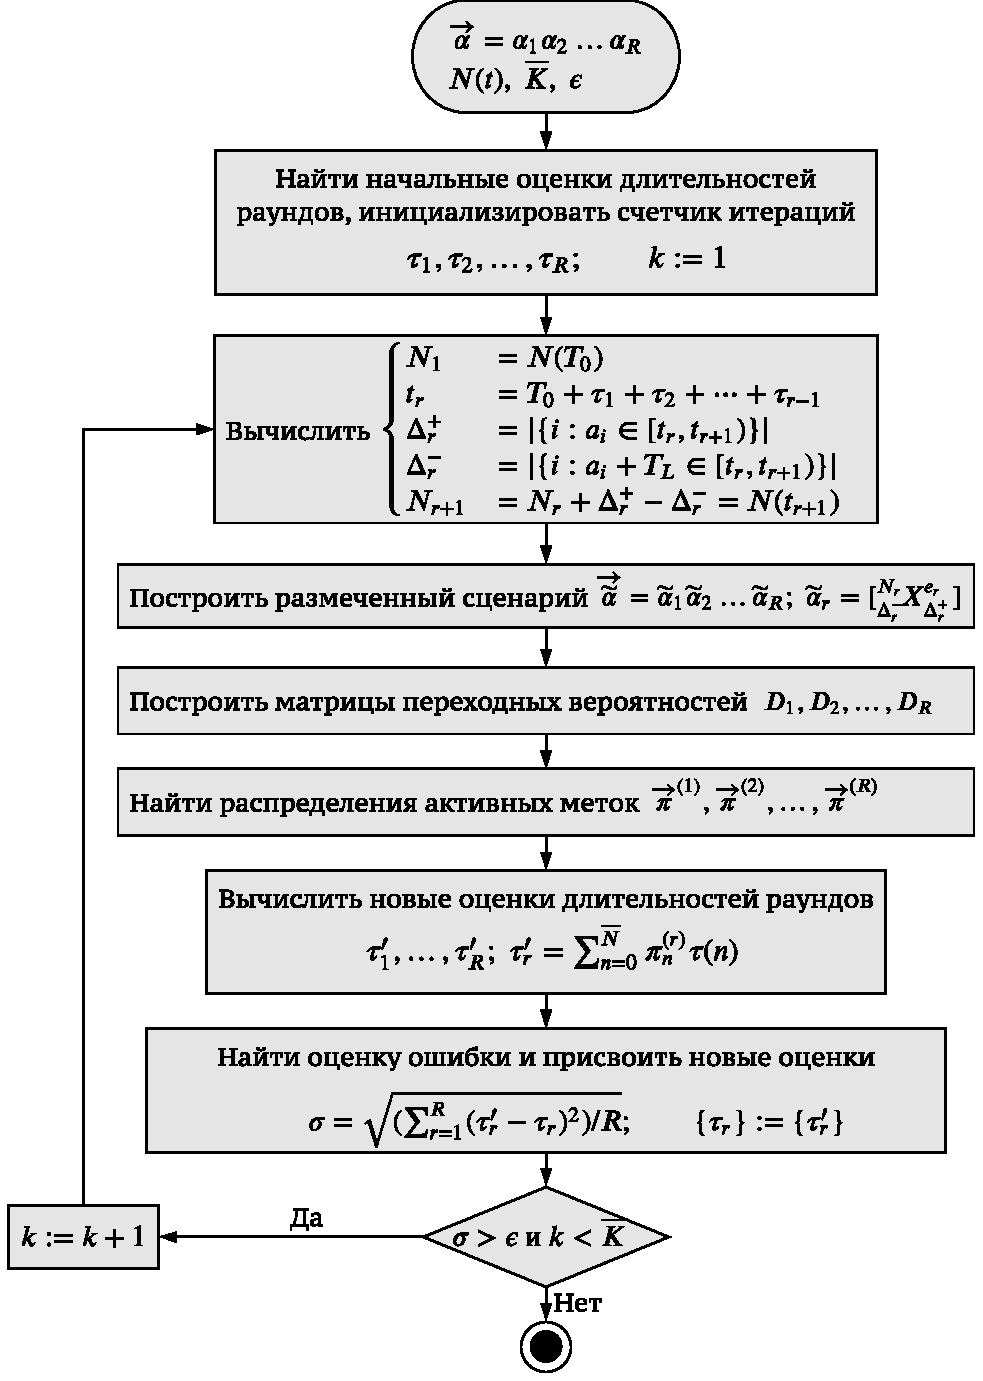
\includegraphics[width=0.7\textwidth]{chapter3/ch3_iterative_algorithm}
  }
  \caption{Итерационный алгоритм расчета длительностей раундов.}
  \label{fig:ch3_iterative_algorithm}
\end{figure}

\textit{Шаг 1}. Произвольно выбираются начальные оценки длительностей раундов $\tau_1, \tau_2, \dots, \tau_R$, а счетчик числа итераций $k$ выставляется равным единице.

\textit{Шаг 2}. Вычисляется число меток в системе в начале первого раунда $N_1$, время начала каждого раунда $t_r = T_0 + \tau_1 + \tau_2 + \cdots + \tau_{r-1}$, число поступивших и покинувших систему за $r$-й раунда меток $\Delta_r^+ = |\{i: t_r \leqslant a_i < t_{r+1}\}|$ и $\Delta_r^- = |\{i: t_r \leqslant a_i + T_L < t_{r+1} \}|$. Затем вычисляется число меток во втором и последующих раундах $N_r = N_{r-1} + \Delta_{r-1}^+ - \Delta_{r-1}^-$ (это же число можно получить как $N_r = N(t_r)$).

\textit{Шаг 3}. По найденным значениям $\{ N_r \}$, $\{ \Delta_r^+ \}$, $\{ \Delta_r^- \}$ и заданному сценарию $\bm{\alpha} = \alpha_1 \alpha_2 \dots \alpha_R$ строится размеченный сценарий $\widetilde{\bm{\alpha}} = \widetilde{\alpha}_1 \widetilde{\alpha}_2 \dots \widetilde{\alpha}_R$, $\widetilde{\alpha}_r = [\prescript{N_r}{\Delta_r^-} X^{e_r}_{\Delta_r^+}]$.

\textit{Шаг 4}. С помощью найденного размеченного сценария строятся матрицы переходных вероятностей $D_1, D_2, \dots, D_R$ процесса $\{ \eta_r \}_{r=1}^\infty$. Для нахождения матриц $D_r$ (см. блок-схему на рис.~\ref{fig:ch3_matrix_composition}) используются матрицы элементарных операций, которые задаются выражениями \eqref{eq:ch3_bg_inventory},~\eqref{eq:ch3_bg_switch},~\eqref{eq:ch3_bg_power_off},~\eqref{eq:ch3_bg_tag_arrival} и \eqref{eq:ch3_bg_tag_departure}.

\textit{Шаг 5}. Вычисляется стационарное распределение числа активных меток перед каждым раундом $\bm{\pi}^{(1)}, \bm{\pi}^{(2)}, \dots, \bm{\pi}^{(R)}$ как решение системы линейных алгебраических уравнений \eqref{eq:ch3_bg_pmf_system}.

\textit{Шаг 6}. С помощью найденных распределений вероятностей $\{ \bm{\pi}^{(r)} \}_{r=1}^R$ вычисляются новые оценки длительностей раундов $\tau'_1, \tau'_2, \dots, \tau'_R$, где $\tau'_r = \sum_{n=0}^{\overline{N}} \pi^{(r)}_n \tau(n)$, а длительность раунда для заданного числа активных меток $\tau(n)$ вычисляется с помощью \eqref{eq:ch3_round_duration_of_n}.

\textit{Шаг 7}. Вычисляется среднеквадратичное отклонение между предыдущей и новой оценкой длительностей раундов $\sigma = \sqrt{\sum_{r=1}^R (\tau'_r - \tau_r)^2 / R}$. Если $\sigma \leqslant \epsilon$ или число итераций $k$ достигло максимального $\overline{K}$, то последние вычисленные оценки $\{ \tau'_r \}_{r=1}^R$ возвращаются в качестве результата выполнения алгоритма, и он завершается. В противном случае, если $\sigma > \epsilon$ и $k < \overline{K}$, счетчик числа итераций $k$ увеличивается на единицу, найденные оценки $\{ \tau'_r \}$ используются вместо исходных $\{ \tau_r \}$, и алгоритм переходит на шаг 2.

Следует сделать несколько замечаний относительно работы алгоритма. Во-первых, в общем случае алгоритм может не сойтись к определенному набору значений $\{ \tau_r \}_{r=1}^R$ со сколь угодно малой точностью. Это связано с возможным зацикливанием: при одной оценке события изменения числа меток происходят в одних раундах, при пересчете оценок "--- в других; но после еще одной или нескольких переоценок длительностей изменения числа меток опять начинают происходить в тех же раундах, что и ранее. Для того, чтобы алгоритм наверняка завершался, введено ограничение на число итераций. Отметим, что в ходе интенсивных численных экспериментов алгоритм завершался всегда, причем в подавляющем большинстве случаев ему хватало всего двух итераций.

Во-вторых, в качестве входа стоит использовать не сам сценарий $\bm{\alpha} = \alpha_1 \alpha_2 \dots \alpha_R$, а его многократно увеличинную версию вида
$$
	\bm{\alpha}^{[L]} = \underbrace{\bm{\alpha} \dots\, \bm{\alpha}}_{L \text{ повторов}} =
		\underbrace{\alpha_1 \dots\, \alpha_R \; \alpha_1 \dots\, \alpha_R\; \dots \, \alpha_1 \dots\, \alpha_R}_{LR \text{ символов}}.
$$
Это приходится делать для того, чтобы в моделируемый участок времени попало достаточное число событий поступления и выхода меток из системы, так как обычно $a_{i+1} - a_i \gg \tau_{max}$. Чем больше $L$, тем точнее будут полученные результаты. Нужно, однако, учесть, что увеличение длины сценария ведет к увеличению времени расчета.

В-третьих, желательно начинать моделирование с того момента $T_0$, когда в системе уже находится некоторое количество меток. Так как переходная матрица $D_R$ строится по символам расширенного сценария $\widetilde{\alpha}_R = [\prescript{N_R}{\Delta_R^-} X^{e_R}_{\Delta_R^+}]$ и $\widetilde{\alpha}_1 = [\prescript{N_1}{\Delta_1^-} Y^{e_1}_{\Delta_1^+}]$, то если начинать моделирования с момента $T_0 = 0$, для которого $N(T_0) = 0$, а в среднем в системе находится $N_a = \lim_{T \rightarrow \infty} \frac{1}{T} \int_{t=0}^{T} N(t) dt > 1$ меток, то в результате перехода вся информация о том, в каких состояниях находились метки, потеряется, и распределение вероятностей будет $\bm{\pi}^{(R+1)} \equiv \bm{\pi}^{(0)} \equiv (1, 0, \dots, 0)$; все метки после $R$-го раунда как будто внезапно исчезнут из системы. Чтобы этого избежать, желательно начинать моделирование с некоторго момента $T_0$, в который $N(T_0) \approx N_a$. Например, если метки поступают через равные промежутки времени $\Delta t$, можно выбрать такой момент, когда в области чтения находится $\lfloor T_L / \Delta t \rfloor$ меток.

После того, как найдены оценки длительностей раундов $\{ \tau_r \}$, числа меток в системе в начале каждого раунда $\{ N_r \}$ и числа покидающих и поступающих меток $\{ \Delta_r^- \}$ и $\{ \Delta_r^+ \}$, можно рассчитать вероятность идентификации отдельной метки.






%%%%%%%%%%%%%%%%%%%%%%%%%%%%%%%%%%%%%%%%%%%%%%%%%%%%%%%%%%%%%%%%%%%%%%%%%%%%%%%%
\section{Расчет вероятности идентификации}
%%%%%%%%%%%%%%%%%%%%%%%%%%%%%%%%%%%%%%%%%%%%%%%%%%%%%%%%%%%%%%%%%%%%%%%%%%%%%%%%
После выполнения итерационного алгоритма, известны оценки длительностей раундов $\{ \tau_r \}_{r=1}^R$, размеченный сценарий $\widetilde{\bm{\alpha}} = \widetilde{\alpha}_1 \widetilde{\alpha}_2 \dots \widetilde{\alpha}_R$, $\widetilde{\alpha}_r = [\prescript{N_r}{\Delta_r^-} X^{e_r}_{\Delta_r^+}]$ и распределения числа активных меток в каждом раунде $\{ \bm{\pi}^{(r)} \}_{r=1}^R$. Для расчета вероятности идентификации рассмотрим проезд области чтения одной выделенной меткой. Система при этом ведет себя как обычно: считыватель работает, а метки поступают и покидают систему по сценарию $\bm{\widetilde{\alpha}}$. Выберем такой раунд $r_0$, что $\Delta_{r_0-1}^+ > 0$, то есть перед раундом $r_0$ в систему поступила новая метка. Время нахождения метки в области известно и равно $T_L$ по условию задачи. Определим число $Q_{r_0}$ как количество раундов, в течение которых метка, поступившая в раунде $r_0$ находится в системе, то есть:

$$
\tau_{r_0} + \tau_{r_0 + 1} + \dots + \tau_{r_0 + Q_{r_0} - 2} < T_L \leqslant \tau_{r_0} + \tau_{r_0 + 1} + \dots + \tau_{r_0 + Q_{r_0} - 1},
$$
где $\tau_{r} \equiv \tau_{(r - 1)(\textbf{mod } R) + 1}$, то есть $\tau_{R+1} \equiv \tau_1$, $\tau_{R+2} \equiv \tau_2$ и так далее.

Рассмотрим конечный двумерный случайный процесс $\{ (\eta_r^{[r_0]}, \phi_r^{[r_0]}) \}_{r=1}^{Q_{r_0}}$, в котором $\eta_r^{[r_0]} \equiv \eta_{r+r_0-1}$ "--- число активных меток в $(r + r_0 - 1)$-м раунде, а $\phi_r$ "--- состояние выделенной метки: если метка еще ни разу не передала успешно свой идентификатор (EPCID или TID), то $\phi_r^{[r_0]} = 0$, если метка неактивна, и $\phi_r^{[r_0]} = 1$, если активна. Если же выделенная метка хотя бы раз успешно передала свой идентификатор, то $\phi_r^{[r_0]} = 2$ независимо от того, активна ли она, то есть $\phi_r^{[r_0]} = 2$ "--- поглощающее состояние процесса $\{ \phi_r \}$. Вероятность идентификации наблюдаемой метки при условии, что она поступила в раунде $r_0$, можно выразить как $\mathbb{P}\{ \phi_{Q_{r_0}}^{[r_0]} = 2\}$.

Номер раунда $r_0$, в котором поступила наблюдаемая метка, определяется не однозначно. Разумно предположить, что вероятность выбора такого раунда пропорциональна его длительности. Положим $\Delta_0^+ = \Delta_R^+$ и обозначим множество всевозможных номеров раундов, в которых происходило увеличение числа меток в системе, как $\mathfrak{R}$:

$$
	\mathfrak{R} = \{ r\:|\:r \in [1, R],\; \Delta_{r-1}^+ > 0 \},
$$
а вероятность поступления метки в раунде $r_0 \in \mathfrak{R}$ оценим как:
\begin{equation}\label{eq:ch3_fg_prob_arrival}
	p^{[a]}_{r_0} = \frac{\tau_{r_0}}{\sum_{r \in \mathfrak{R}} \tau_r}
\end{equation}
Используя введенные обозначения, вероятность идентификации метки можно выразить с помощью полной вероятности:
\begin{equation}\label{eq:ch3_tag_id_prob_phi}
	P_X = \sum\limits_{r \in \mathfrak{R}} p^{[a]}_r \mathbb{P}\{ \phi^{[r]}_{Q_r} = 2 \}.
\end{equation}

Таким образом, для нахождения вероятности идентификации метки нужно найти вероятности идентификации метки $\mathbb{P}\{ \phi^{[r_0]}_{Q_{r_0}} = 2 \}$ при условии поступления ее в раунде $r_0 \in \mathfrak{R}$. Стоит отметить, что процесс $\{ \phi^{[r_0]}_r \}$ не является марковским, так как вероятности его переходов между состояниями 0 и 1 зависят не только от его текущего состояния, но и от того, сколько в системе активных меток. Например, если $\phi_r^{[r_0]} = 0$ (наблюдаемая метка неактивна) и других активных меток в системе нет, то вероятность перехода $\phi_r^{[r_0]}$ в состояние 1 или 2 определяется только вероятностью успешной передачи ответа RN16 меткой в очередном раунде; если же в системе есть активные метки, то нужно также учитывать вероятность коллизий.



%%% --------------------------------------------
% \subsection{Определение основного процесса \texorpdfstring{\( \{ \gamma_r \} \)}{γ\_\{r\}}}
\subsection{Определение основного процесса}
%%% --------------------------------------------
% \subsection{Заголовки с формулами: \texorpdfstring{\(a^2 + b^2 = c^2\)}{%
% a\texttwosuperior\ + b\texttwosuperior\ = c\texttwosuperior},
% \texorpdfstring{\(\left\vert\textrm{{Im}}\Sigma\left(
% \protect\varepsilon\right)\right\vert\approx const\)}{|ImΣ (ε)| ≈ const},
% \texorpdfstring{\(\sigma_{xx}^{(1)}\)}{σ\_\{xx\}\textasciicircum\{(1)\}}
% }\label{subsec:with_math}

Рассмотрим двумерный процесс $\{ (\eta_r^{[r_0]}, \phi_r^{[r_0]}) \}_{r=1}^{Q_{r_0}}$. Во всех дальнейших расчетах вплоть до вычисления вероятности $P_X$ будем использовать процесс, начинающийся в раунде $r_0$, поэтому, для сокращения записи, будем опускать верхний индекс $[r_0]$, но подразумевать его. Таким образом, вместо $\phi_r^{[r_0]}$ будем писать $\phi_r$, вместо $Q_{r_0}$ "--- просто $Q$ и так далее.

\begin{figure}[htb]
	\centerfloat{
    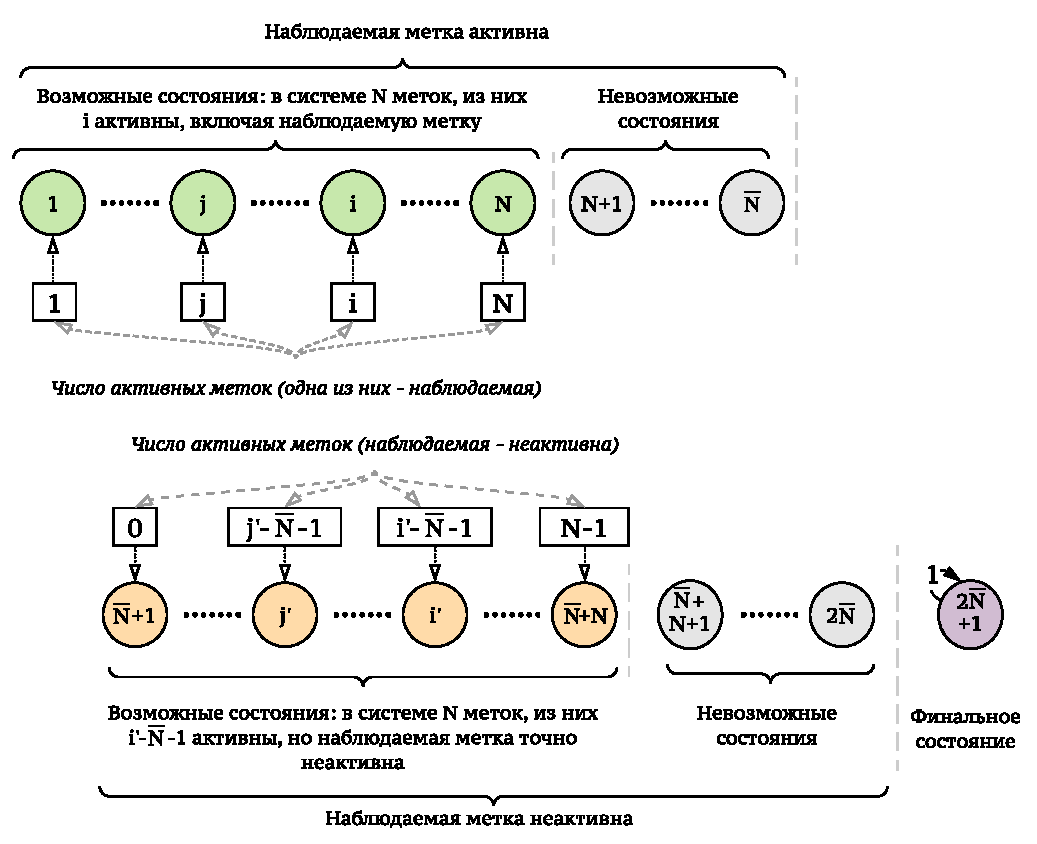
\includegraphics[width=0.9\textwidth]{chapter3/ch3_fg_structure}
  }
  \caption{Структура пространства состояний основного процесса $\{\gamma_r\}$, когда в системе $N$ меток.}
  \label{fig:ch3_fg_structure}
\end{figure}

Изменения компонентов процесса $\{ (\eta_r, \phi_r) \}$ не являются независимыми. Например, если $\eta_r = 0$, вероятность того, что $\phi_r = 1$ равна нулю: наблюдаемая метка не может быть активной, если активных меток в системе нет. Чтобы избавиться от недостижимых состояний вместо двумерного процесса будем рассматривать одномерный процесс $\{ \gamma_r \}_{r=1}^Q$, $\gamma_r \in [1, 2\overline{N}+1]$ (см. рис.~\ref{fig:ch3_fg_structure}), в котором:

\begin{equation}\label{eq:ch3_gamma_process}
	\begin{aligned}
		1 \leqslant \gamma_r \leqslant \overline{N}                 &\Leftrightarrow \phi_r = 1 \text{ и } \eta_r = \gamma_r \\
		\overline{N} + 1 \leqslant \gamma_r \leqslant 2\overline{N} &\Leftrightarrow \phi_r = 0 \text{ и } \eta_r = \gamma_r - \overline{N} - 1\\
		\gamma_r = 2\overline{N}+1                                  &\Leftrightarrow \phi_r = 2
	\end{aligned}
\end{equation}

Попадание в состояние $\gamma_r = 2\overline{N} + 1$ означает, что наблюдаемая метка успешно передала свой идентификатор, это состояние является поглощающим. При $\gamma_r \leqslant \overline{N}$ число активных меток $\eta_r$ равно $\gamma_r$, причем наблюдаемая метка активна. Если же процесс $\gamma_r$ находится в состоянии из интервала $[\overline{N}+1, 2\overline{N}]$, то наблюдаемая метка неактивна, и число активных меток $\eta_r$ определяется как $\gamma_r - (\overline{N}+1)$. Легко видеть, что для состояний $\eta_r = 0, \phi_r = 1$ (активных меток в системе нет, но наблюдаемая метка активна), а также $\eta_r = \overline{N}, \phi_r = 0$ (все метки активны, но наблюдаемая метка неактивна), нет соответствующих состояний $\gamma_r$; кроме того, значения $\eta_r$ неразличимы при $\gamma_r = 2\overline{N} + 1$.

Переходные вероятности для процесса $\{ \gamma_r \}$ найдем аналогично тому, как ранее определялись переходные вероятности для случайного процесса $\{ \eta_r \}_{r=1}^\infty$: сначала покажем, что вероятности переходов $\{ \gamma_r \}$ при выполнении элементарных операций зависят только от текущего состояния и выпишем их, а затем покажем, как построить матрицы переходных вероятностей между раундами.



%%% --------------------------------------------
% \subsection{Переходные вероятности процесса \texorpdfstring{\( \{ \gamma_r \} \)}{γ\_\{r\}} для элементарных операций}
\subsection{Переходные вероятности основного процесса для элементарных операций}
%%% --------------------------------------------
Для обозначений переходных вероятностей процесса $\{ \gamma_r \}$ при выполнении элементарных операций будем использовать нотацию, аналогичную обозначениям для процесса $\{ \eta_r \}$ ($U_N^{\nabla}, U_N^{\times}, \dots$), но вместо буквы $U$ использовать $V$. Как и в разделе \ref{subsec:ch3_bg_elem_op_matrices}, здесь для удобства будем предполагать, что состояние процесса $\{ \gamma_r \}$ изменяется при выполнении одной из элементарных операций: инвентаризации ($V_N^\nabla$), смены флага ($V_N^\times$), сброса питания ($V_N^\downarrow$), добавления или удаления метки ($V^+_{X,N}$ и $V^-_N$ соответственно). В дальнейшем же шаг процесса будет, как обычно, соответствовать раунду.

Пусть $V$ "--- одна из элементарных операций, состояние процесса $\gamma_r$ перед ее выполнением есть $\gamma_r = i$, а после "--- $\gamma_{r+1} = j$, $i,j \in [1,\;2\overline{N}+1]$. Как и ранее для процесса $\{ \eta_r \}$, в силу сделанных допущений, в частности "--- о постоянстве BER во всей области чтения, каждую элементарную операцию можно задать распределением вероятностей $\mathbb{P}\{\gamma_{r+1} = j | \gamma_r = i\}$. Эти вероятности определяются аналогично тому, как это было сделано для переходных вероятностей $\{ \eta_r \}$, однако здесь приходится отдельно рассматривать переходы при $\phi_r = 0$ и $\phi_r = 1$. Рассмотрим переходные матрицы $V \in \mathbb{R}^{(2\overline{N}+1) \times (2\overline{N}+1)}$ каждой из элементарных операций (см. рис.~\ref{fig:ch3_bg_trans}). Как и в разделе $\ref{subsec:ch3_bg_elem_op_matrices}$, некорркетные состояния $j \in [N+1, \overline{N}] \cup [\overline{N} + N + 1,\; 2\overline{N}]$, которые соответствуют $\eta_r > N$ (то есть в которых активных меток больше, чем всего меток в системе), не будут достижимы из корректных состояний $i \in [1,\;N] \cup [\overline{N}+1,\;\overline{N} + N]$, а у них самих будут только переходы-петли с вероятностью 1. Единственное исключение из этого правила "--- операция добавления метки $V_{A,N}^+$. Переходные вероятности при выполнении элементарных операций показаны на рис.~\ref{fig:ch3_fg_trans_inventory} и рис.~\ref{fig:ch3_fg_trans}.

\begin{figure}[htb]
	\centerfloat{
    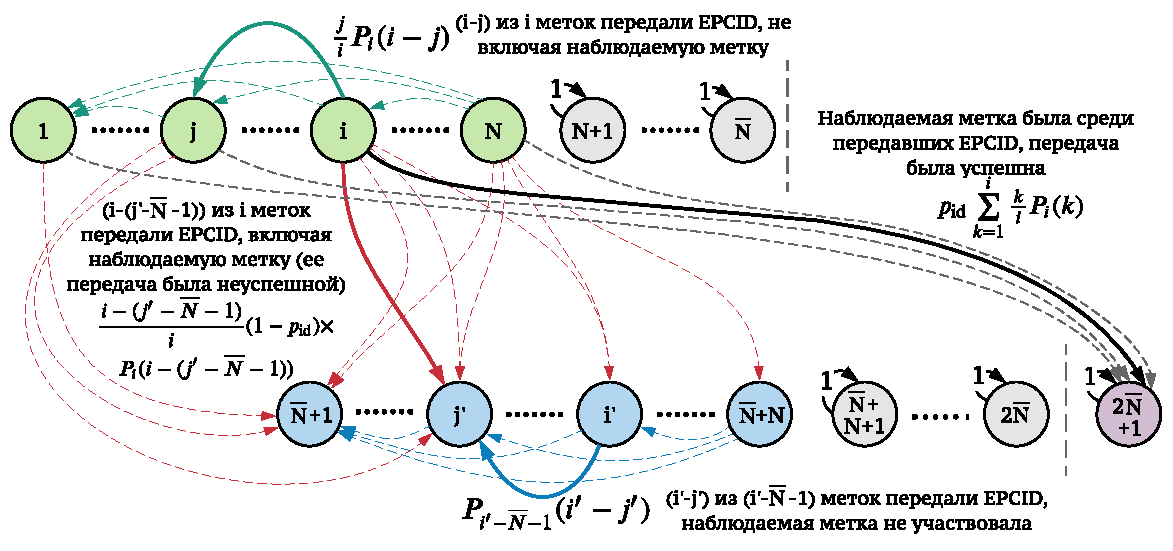
\includegraphics[width=0.9\textwidth]{chapter3/ch3_fg_trans_inventory}
  }
  \caption{Переходные вероятности основного процесса $\{\gamma_r\}$ при выполнении операции инвентаризации $V^\nabla_N$.}
  \label{fig:ch3_fg_trans_inventory}
\end{figure}

Применение операции опроса меток $V_N^\nabla$ приводит к тому, что часть активных меток успешно передают RN16 и затем пытаются передать EPCID. Если одной из таких меток оказалась наблюдаемая метка (то есть $n \leqslant \overline{N}$), то процесс может перейти в поглощающее состояние, если наблюдаемая метка сможет полностью передать свой идентификатор. Если же ей это не удастся, то она может либо остаться активной (случай неуспешной передачи RN16), либо инвертировать флаг, но ошибиться уже после передачи RN16. При построении вероятностей удобно рассматривать три независимых события: $(i - j)$ из $i$ активных меток успешно передали свои RN16 (вероятность $P_i(i - j)$); наблюдаемая метка попала в число меток, успешно передавших RN16 (вероятность $(i - j)/i$); наблюдаемая метка успешно передала свой идентификатор (вероятность $p_{\text{id}}$). С учетом этого замечания и определения состояний процесса $\{ \gamma_r \}$ (см.~\eqref{eq:ch3_gamma_process}), вероятности определяются следующим образом (см. рис.~\ref{fig:ch3_fg_trans_inventory}):

\begin{equation}\label{eq:ch3_fg_inventory}
	\{ V^\nabla_N \}_{ij} = \begin{cases}
		\frac{j}{i}P_i(i - j), &1 \leqslant j \leqslant i \leqslant N\\
		P_{i-\overline{N}-1}(i - j), &\overline{N} + 1 \leqslant j \leqslant i \leqslant \overline{N}+N\\
		\mathrlap{\frac{i - (j - \overline{N} - 1)}{i} (1 - p_{\text{id}}) P_i(i - (j - \overline{N} - 1)),}\\
			\mathrlap{\quad\qquad\qquad\qquad 1 \leqslant i \leqslant N, \; \overline{N}+1 \leqslant j \leqslant \overline{N} + N}\\
		p_{\text{id}} \sum_{k = 1}^i \frac{k}{i} P_i(k), & 1 \leqslant i \leqslant N,\; j = 2\overline{N}+1\\
		1, & N < i = j \leqslant \overline{N}\\
		1, & \overline{N} + N < i = j \leqslant 2\overline{N}+1\\
		0, &\text{в остальных случаях.}
 	\end{cases}
\end{equation}

\begin{figure}[htb]
	\centerfloat{
    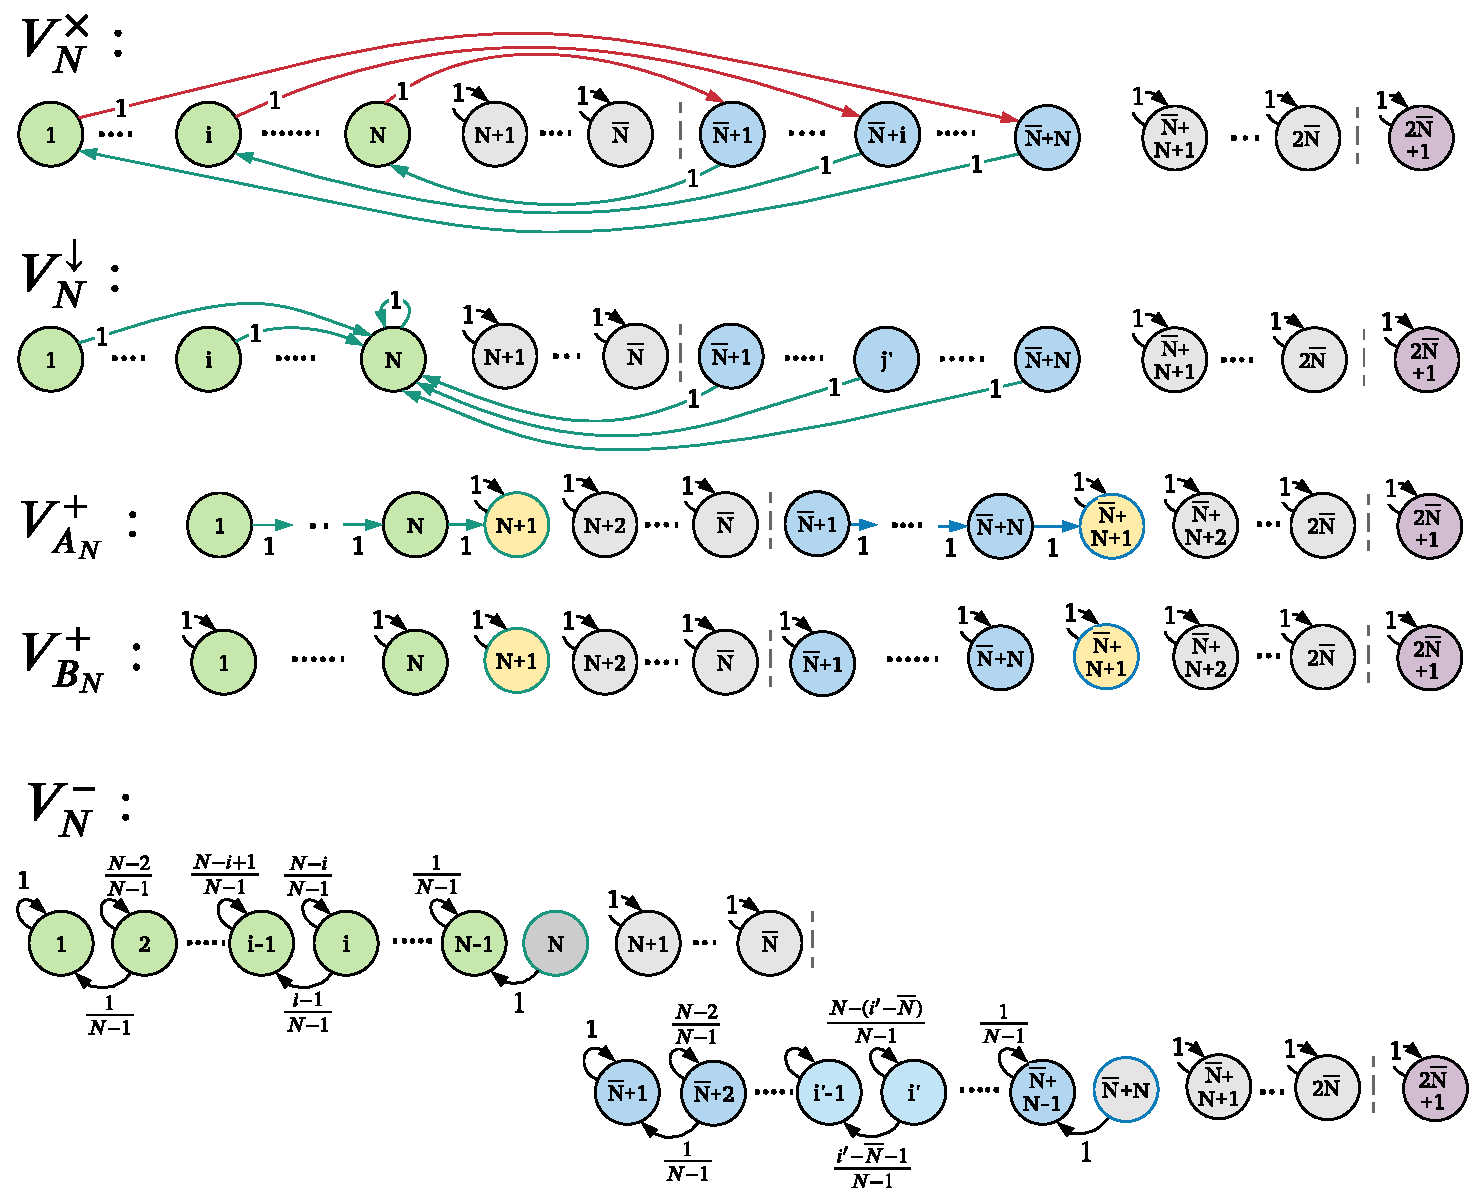
\includegraphics[width=0.9\textwidth]{chapter3/ch3_fg_trans}
  }
  \caption{Переходные вероятности основного процесса $\{\gamma_r\}$ при выполнении элементарных операций.}
  \label{fig:ch3_fg_trans}
\end{figure}

При смене флага $V_N^\times$ активные и неактивные метки меняются местами. Это справедливо и для наблюдаемой метки, поэтому значение $\phi_r$ меняется с 1 на 0 и обратно. Учитывая определение \eqref{eq:ch3_gamma_process}, получаем следующие значения переходных вероятностей (см. рис.~\ref{fig:ch3_fg_trans}):

\begin{equation}\label{eq:ch3_fg_switch}
	\{ V_N^\times \}_{ij} = \begin{cases}
 		1, & 1 \leqslant i \leqslant N, \; j = \overline{N} + N + 1 - i\\
 		1, & \overline{N} + 1 \leqslant i \leqslant \overline{N} + N,\; j = N - (i - \overline{N} - 1)\\
 		1, & N < i = j \leqslant \overline{N}\\
 		1, & \overline{N} + N < i = j \leqslant 2\overline{N} + 1\\
 		0, & \text{в остальных случаях.}
 	\end{cases}
\end{equation}

В результате выключения питания $V_N^\downarrow$ все метки сбрасывают свои флаги в $A$, на него же переключается считыватель. Поэтому из любого корректного непоглощающего состояния $i \in [1, N] \cup [\overline{N}+1, \overline{N} + N]$ операция переводит процесс в состояние $\gamma_{r+1} = N$:

\begin{equation}\label{eq:ch3_fg_power_off}
	\{ V_N^\downarrow \}_{ij} = \begin{cases}
 		1, & 1 \leqslant i \leqslant N,\; j = N\\
 		1, & \overline{N}+1 \leqslant i \leqslant \overline{N} + N,\; j = N\\
 		1, & N < i = j \leqslant \overline{N}\\
 		1, & \overline{N} + N < i = j \leqslant 2\overline{N} + 1\\
 		0, & \text{в остальных случаях}.
 	\end{cases}
\end{equation}

Операции добавления метки $V_{A,N}^+$ и $V_{B,N}^+$ никак не влияют на состояние наблюдаемой метки $\phi_r$ и изменяют число активных меток только в том случае, если текущий флаг опроса равен $A$:

\begin{equation}\label{eq:ch3_fg_tag_arrival}
	\begin{aligned}
		\{ V_{A_N}^+ \}_{ij} &= \begin{cases}
 			1, & 1 \leqslant i \leqslant N,\; j = i + 1\\
 			1, & \overline{N}+1 \leqslant i \leqslant \overline{N} + N ,\; j = i + 1\\
	 		1, & N < i = j \leqslant \overline{N}\\
 			1, & \overline{N} + N < i = j \leqslant 2\overline{N} + 1\\
 			0, & \text{в остальных случаях}
	 	\end{cases}\\
	 	V_{B_N}^+ &= I_{2\overline{N}+1}
	\end{aligned}
\end{equation}
Здесь $I_{2\overline{N}+1}$ "--- единичная матрица порядка $2\overline{N}+1$.

При моделировании выхода метки из области чтения $V_N^-$ будем предполагать, что выйти может любая из меток, кроме наблюдаемой\footnote{Отметим, что из-за этого допущения возможна некоторая неточность, так как в действительности метки выходят в соответствии с их законом движения, и вероятность выхода метки с определенным флагом $X$ может не быть равна отношению числа меток с флагом $X$ к общему числу меток; но это допущение существенно упрощает модель и позволяет не учитывать положения меток.}. Про наблюдаемую же метку заведомо известно, что она остается в системе, поэтому при расчете вероятностей ее учитывать не нужно. В остальном, вероятности определяются так же, как и в~\eqref{eq:ch3_bg_tag_departure}, с поправкой на структуру состояний $\{ \gamma_r \}$ (см. рис.~\ref{fig:ch3_fg_trans}).

\begin{equation}\label{eq:ch3_fg_tag_departure}
	\{ V_N^- \}_{ij} = \begin{cases}
 		\frac{i-1}{N-1}, & 1 < i \leqslant N,\; j = i - 1\\
 		\frac{N-i}{N-1}, & 1 \leqslant i = j \leqslant N\\
 		\frac{i - \overline{N} - 1}{N - 1}, & \overline{N} + 1 < i \leqslant \overline{N} + N,\; j = i - 1\\
 		\frac{N - (i - \overline{N})}{N - 1},  & \overline{N} + 1 \leqslant i = j \leqslant \overline{N} + N\\
 		1,               & N < i = j \leqslant \overline{N}\\
 		1,               & \overline{N} + N < i = j \leqslant 2\overline{N} + 1\\
 		0,               & \text{в остальных случаях}.
 	\end{cases}
\end{equation}





%%% --------------------------------------------
% \subsection{Матрицы переходных вероятностей между раундами для процесса \texorpdfstring{\( \{ \gamma_r \} \)}{γ\_\{r\}}}
\subsection{Матрицы переходных вероятностей между раундами для основного процесса}
%%% --------------------------------------------
Здесь и далее будем считать, что состояние процесса $\{ \gamma_r \}$ меняется между раундами, а не между элементарными операциями. Рассмотрим размеченный сценарий $\widetilde{\bm{\alpha}} = \widetilde{\alpha}_1 \widetilde{\alpha}_2 \dots \widetilde{\alpha}_R$, $\widetilde{\alpha}_r = [\prescript{N_r}{\Delta_r^-} X^{e_r}_{\Delta_r^+}]$. Будем считать, что наблюдаемая метка поступила в раунде $r_0$, для которого $\Delta_{r_0}^+ > 0$, и находилась в системе в течение $Q_{r_0}$ раундов. Тогда для наблюдаемой метки работа считывателя будет задаваться размеченным сценарием $\widetilde{\bm{\alpha}}^{[r_0]} = \widetilde{\alpha}_1^{[r_0]} \widetilde{\alpha}_2^{[r_0]} \dots \widetilde{\alpha}_{Q_{r_0}}^{[r_0]}$, где $\widetilde{\alpha}_i^{[r_0]} \equiv \widetilde{\alpha}_{r_0 + i - 1}$. Обозначим матрицы переходных вероятностей процесса $\{ \gamma_r^{[r_0]} \}$ между раундами $r$ и $r+1$, как $C_r^{[r_0]}$.

Пусть $\widetilde{\alpha}_r^{[r_0]} = (X, N, e, \Delta^-, \Delta^+)$ и $\widetilde{\alpha}_{r+1}^{[r_0]} = (Y, \bullet, \bullet, \bullet, \bullet)$ (здесь $\bullet$ "--- произвольное значение). Как и переходная матрица $D_r$ фонового процесса $\{ \eta_r \}$, матрица переходных вероятностей основного процесса $C_r^{[r_0]}$ определяется значениям $X$, $N$, $e$, $\Delta^+$, $\Delta^-$ и $Y$, и ее можно получить как произведение матриц элементарных операций $V_N^\nabla$, $V_N^\times$, $V_N^\downarrow$, $V_{X,N}^+$, $V_N^-$. Для этого можно использовать алгоритм, описанный в разделе~\ref{subsec:ch3_bg_op_composition} и показанный на рис.~\ref{fig:ch3_matrix_composition}, заменяя матрицы $U_N^\nabla, U_N^\times, U_N^\downarrow, U_{X,N}^+, U_N^-$ на матрицы элементарных операций для основного процесса $V_N^\nabla, V_N^\times, V_N^\downarrow, V_{X,N}^+, V_N^-$.



%%% --------------------------------------------
% \subsection{Расчет вероятности поглощения процесса \texorpdfstring{\( \{ \gamma_r \} \)}{γ\_\{r\}}}
\subsection{Расчет вероятности поглощения процесса}
%%% --------------------------------------------
Зная переходные вероятности процесса $\{ \gamma_r^{[r_0]} \}$, можно вычислить вероятность того, что метка, поступивашая в систему в раунде $r_0 \in \mathfrak{R}$ успешно передаст свой идентификатор. Обозначим $\bm{\theta}^{(r_0,r)} \in \mathbb{R}^{2\overline{N}+1}$ распределение вероятностей процесса $\gamma_r^{[r_0]}$ на $r$-м шаге, а $\bm{\theta}^{(r_0,1)}$ "--- его начальное распределение. Так как вероятности переходов между $r$-м и $(r+1)$-м раундами определяются матрицей $C_r^{[r_0]}$, то
$$
\bm{\theta}^{(r_0,r+1)} = \bm{\theta}^{(r_0,r)} C_{r}^{[r_0]} = \bm{\theta}^{(r_0,1)} C_1^{[r_0]} C_2^{[r_0]} \dots C_r^{[r_0]}.
$$
В частности, распределение вероятностей после $Q_{r_0}$ раундов можно вычислить как:
$$
\bm{\theta}^{(r_0, Q_{r_0} + 1)} = \bm{\theta}^{(r_0, 1)} C^{[r_0]}_1 C^{[r_0]}_2 \dots C^{[r_0]}_{Q_{r_0}}.
$$

В силу определения состояний процесса $\{ \gamma_r^{[r_0]} \}$ \eqref{eq:ch3_gamma_process}, вероятность попадания процесса $\{ \phi_r^{[r_0]} \}$ в поглощающее состояние $\phi_r^{[r_0]} = 2$ тождественно равна вероятности попадания процесса $\{ \gamma_r^{[r_0]} \}$ в его поглощающее состояние $\gamma_{Q_{r_0}}^{[r_0]} = 2\overline{N}+1$, то есть
$$
	\mathbb{P}\{ \phi_{Q_{r_0}}^{[r_0]} = 2 \} \equiv \mathbb{P}\{ \gamma_{Q_{r_0}}^{[r_0]} = 2\overline{N}+1 \} = \theta_{2\overline{N}+1}^{(r_0, Q_{r_0}+1)}.
$$

Таким образом, для вычисления вероятности поглощения процесса $\{ \phi_r^{[r_0]} \}$, то есть успешной идентификации наблюдаемой метки, поступившей в систему в раунде $r_0$, нужно вычислить распределение вероятностей после выполнения $Q_{r_0}$ раундов. Так как размеченный сценарий $\widetilde{\bm{\alpha}}$, по которому строятся матрицы переходных вероятностей $C^{[r_0]}_1$, $C^{[r_0]}_2$, $\dots$, $C^{[r_0]}_{Q_{r_0}}$, был построен одновременно с вычислением оценок длительностей раундов $\tau_1, \tau_2, \dots, \tau_R$ в результате выполнения итерационного алгоритма (см. раздел~\ref{subsec:ch3_iterative_algorithm}), то неизвстным остается только начальное распределение $\bm{\theta}^{(r_0, 1)}$.

Для нахождения начального распределения $\bm{\theta}^{(r_0,1)}$ нужно учесть, что об этом распределении уже кое-что известно. Во-первых, известно, будет ли наблюдаемая метка активна сразу после поступления: она будет активной, если и только если в раунде $r_0$ считыватель ведет опрос по флагу $A$, поскольку новая метка всегда хранит флаг со значением $A$. Значит, если $\alpha_{r_0} = A^{e}$, то значение $\phi_1^{[r_0]} = 0$, и, соответственно, $\gamma_1^{[r_0]} \in [1,\; N]$; если же $\alpha_{r_0} = B^{e}$, то $\phi_1^{[r_0]} = 1$ и $\gamma_1^{[r_0]} \in [\overline{N} + 1,\; \overline{N} + N]$ Во-вторых, известно число меток в области чтения $N$ известно, так как известен размеченный сценарий $\widetilde{\bm{\alpha}}$. Наконец, в-третьих, известно распределение числа активных меток $\eta_{r_0}$ в начале раунда $\bm{\pi}^{(r_0)}$ "--- оно было найдено в результате выполнения итерационного алгоритма. Таким образом:
\begin{equation}\label{eq:ch3_fg_initial_prob}
	\theta_n^{(r_0,1)} = \begin{cases}
		\pi^{(r_0)}_n,                      &\widetilde{\alpha}_{r_0} = A^e_N,\; 1 \leqslant n \leqslant N\\
		\pi^{(r_0)}_{n - (\overline{N}+1)}, &\widetilde{\alpha}_{r_0} = B^e_N,\; \overline{N}+1 \leqslant n \leqslant \overline{N}+N\\
		0,                                  &\text{в остальных случаях.}
	\end{cases}
\end{equation}

Подставляя найденные выражения для вероятности попадания $\{ \gamma_r^{[r_0]} \}$ в поглощающее состояние в выражение~\eqref{eq:ch3_tag_id_prob_phi}, получаем, что вероятность идентификации наблюдаемой метки $P_X$ вычисляется так:

$$
	P_X = \sum\limits_{r_0 \in \mathfrak{R}} p_{r_0}^{[a]} \{ \bm{\theta}^{(r_0,1)} C_1^{[r_0]} C_2^{[r_0]} \dots C_{Q_{r_0}}^{[r_0]} \}_{2\overline{N}+1},
$$
где вероятности $p_{r_0}^{[a]}$ вычисляются согласно~\eqref{eq:ch3_fg_prob_arrival}.






%%%%%%%%%%%%%%%%%%%%%%%%%%%%%%%%%%%%%%%%%%%%%%%%%%%%%%%%%%%%%%%%%%%%%%%%%%%%%%%%
\section{Результаты моделирования}
%%%%%%%%%%%%%%%%%%%%%%%%%%%%%%%%%%%%%%%%%%%%%%%%%%%%%%%%%%%%%%%%%%%%%%%%%%%%%%%%
Для численного исследования был выбран простой случай поступления меток через равные интервалы. С помощью аналитической модели исследовались три характеристики:

\begin{itemize}
	\item{распределение числа активных меток по раундам;}
	\item{оценка длительностей раундов;}
	\item{вероятность идентификации отдельной метки.}
\end{itemize}
Первые две характеристики получаются аналитически с помощью фонового процесса, а третья "--- с помощью основного процесса. Для валидации результатов аналитической модели была разработана простая имитационная модель, моделирующая процесс проезда метками области чтения и обмен командами и ответами при постоянном BER. Отметим, что эта модель гораздо проще и быстрее той имитационной модели, которая была описана в предыдущей главе.

Исходный код аналитической и имитационной модели на языке Python 3 с использованием Cython, результаты экспериментов и более подробное описание доступны на GitHub: \url{https://github.com/larioandr/thesis-rfidam}.

Перед тем, как перейти к описанию параметров эксперимента и его результатов, сделаем одно замечание. В коде и выводе неудобно использовать обозначения спецификаций раундов вида $X^e$, которые использовались при построении математической модели. Чтобы избежать верхних индексов и оставить сценарии читаемыми, была использована следующее кодирование в виде строк: если после раунда нет сброса питания, то раунд обозначается только заглавной буквой \texttt{A} или \texttt{B}, а если после раунда считыватель выключается, то после \texttt{A} или \texttt{B} добавляется строчная буква \texttt{x}. Таким образом, сценарий $A^0B^0A^1B^0$ в реализации модели кодируется строкой \texttt{``ABAxB''}.

\subsection{Параметры модели}\label{subsec:ch3_results_params}

Все параметры, которые используются в эксперименте, можно разделить на три группы: \textit{гиперпараметры}, \textit{метапараметры} и \textit{свободные параметры}.

\begin{table}[!t]
	\renewcommand{\arraystretch}{1.3}
	\caption{Параметры модели.}
	\label{table:ch3_results_params}
	\centering
	\begin{tabular}{|l|l|}
		\hline
		Параметр   & Значение \\\hline
		\multicolumn{2}{|c|}{\textit{Гиперпараметры}} \\\hline
		Число моделируемых меток              & 3000  \\\hline
		Кратность расширенных сценариев ($K$) & 2000  \\\hline
		Множитель раундов при свертке ($K_c$) & 3     \\\hline
		\multicolumn{2}{|c|}{\textit{Метапараметры}} \\\hline
		Интервал Tari                              & 12,5~мкс   \\\hline
		Интервал RTcal                             & 37,5~мкс   \\\hline
		Интервал TRcal                             & 56,25~мкс  \\\hline
		Показатель числа слотов (Q)                & 2          \\\hline
		Длительность отключения ($T_\downarrow$)   & 100~мс     \\\hline
		Число символов на бит (M)                  & 2          \\\hline
		Использовать расширенную преамбулу (TRext) & 0 (нет)    \\\hline
		Коэффициент DR ($64/3$ или 8)              & $64/3$     \\\hline
		Длина EPCID                                & 96 бит     \\\hline
		Длина TID                                  & 64 бит     \\\hline
		Время нахождения в области чтения ($T_L$)  & 2,5~сек    \\\hline
		\multicolumn{2}{|c|}{\textit{Свободные параметры}} \\\hline
		Интервалы между поступлениями   & 200~мс, 400~мс, 1~сек \\\hline
		BER                             & от 0 до 0,05 \\\hline
		Сценарии                        & См. в конце раздела~\ref{subsec:ch3_results_params} \\\hline
	\end{tabular}
\end{table}

\textit{Гиперпараметры} влияют на точность результатов и скорость расчетов. В модели используется три гиперпараметра:
\begin{itemize}
	\item число моделируемых меток;
	\item кратность расширенных сценариев;
	\item множитель раундов при свертке.
\end{itemize}
Кратность расширенных сценариев определяет, сколько раз копируется сценарий при построении расширенного сценария (см. раздел~\ref{subsec:ch3_iterative_algorithm}). Чем выше кратность, тем больше моментов поступления и выхода меток попадет в моделируемый (аналитической моделью) интервал, и тем точнее будет результат. Однако при этом растет сложность расчета. Число моделируемых меток определяет, сколько событий поступлений новых меток будет моделироваться в имитационной модели. Множитель при свертке сценариев используется при исследовании характеристик раундов и будет описан подробнее в следующем разделе.

\textit{Метапараметры} - это те величины, которые сами по себе не оказывают существенного влияния на результаты, и для их различных значений можно подобрать диапазоны других (мета- и обычных) параметров, на которых будут получены близкие результаты. Например, так как в модели явно задается BER, то параметр M (число символов на бит в ответах меток) влияет только на длительность сообщений, поэтому, если для M=8 взять большую область чтения и увеличить интервал между метками пропорционально, то можно получить тот же результат, что и для M=1, маленькой области чтения и коротких интервалов между поступлениями. К метапараметрам относятся:

\begin{itemize}
	\item параметры передачи команд считывателя Tari, RTcal, TRcal;
	\item параметры передачи ответов меток M, DR, TRext;
	\item длительность отключения считывателя $T_{\downarrow}$;
	\item время нахождения метки в области чтения $T_L$;
	\item число читаемых слов из TID и размер EPCID в байтах;
	\item показатель числа слотов Q.
\end{itemize}
Отметим, что если бы BER не был свободным параметром (например, свободным параметром был бы SNR), то параметры Tari, M, DR, TRext оказывали бы более существенное влияние и их можно было бы считать свободными, так как от них бы зависел BER. Также отметим, что величина Q влияет на вероятность коллизий, как и число меток в области чтения, а последнее зависит от интервала между поступлениями, который является свободным параметром.

\textit{Свободные параметры} - это те параметры, которые наиболее существенно влияют на результат. К ним относятся:

\begin{itemize}
	\item интервал между поступлениями меток;
	\item сценарий работы считывателя;
	\item вероятность битовой ошибки (BER).
\end{itemize}
При моделировании исследовались четыре группы сценариев:

\begin{itemize}
	\item $A^0$ "--- базовый сценарий без сбросов питания и переключения флагов (<<всегда $A$>>);
	\item $A^0B^0$, $A^0A^0A^0A^0B^0B^0B^0B^0$ "--- сценарии без сброса питания, но с инвертированием флагов опроса;
	\item $A^1$, $A^0A^1$, $A^0A^0A^0A^1$ "--- сценарии без смены флагов, но со сбросом питания;
	\item $A^0B^0A^0B^0$, $A^0A^0A^0A^1A^0B^0A^0B^1$ "--- смешанные сценарии.
\end{itemize}
Значения остальных свободных параметров, а также гиперпараметров и метапараметров приведены в табл.~\ref{table:ch3_results_params}.


\subsection{Анализ свойств раундов}\label{subsec:ch3_results_round_props}

В первую очередь с помощью фонового процесса были получены оценки длительностей раундов и среднее число активных меток в каждом раунде. Также с помощью основного процесса для каждого раунда была найдены оценки вероятности идентификации для меток, поступающих в этом раунде. Для валидации эти значения сравнивались с данными, полученными с помощью имитационного моделирования.

Из-за использования расширенных сценариев в аналитической модели исследуется очень большое число раундов (порядка десяти тысяч). В отличие от аналитики, в имитационной модели один и тот же сценарий (не расширенный) моделируется до тех пор, пока не будет промоделировано достаточное число меток. Так как имитационная модель учитывает положение и состояние конкретных меток, при каждом начале моделирования сценария система будет находиться в новом состоянии. Число раундов в имитационной модели будет много больше, порядка нескольких миллионов. Из-за этого сравнивать оценки длительностей, среднего числа активных меток и вероятности идентификации для каждого отдельного раунда невозможно и нецелесообразно.

Чтобы решить эту проблему и получить наглядное сравнение оценок по раундам, вместо сравнения в каждом отдельном раунде будем сравнивать значения, полученные усреднением по подмножеству раундов, равноотстоящих от начала сценария, то есть ``свернем'' длинный вектор метрик в более короткий. Так как исходный сценарий $\bm{\alpha}$ может быть очень коротким, а расширенный сценарий $\widetilde{\bm{\alpha}}$, используемый в расчетах "--- слишком длинный, будем использовать сценарий $\hat{\bm{\alpha}}$, полученный, как и расширенный сценарий, конкатенацией сценария $\bm{\alpha}$, но меньшее число раз $K_c$. Это число $K_c$ будем называть \textit{множителеми раундов при свертке}. Если кратность расширенных сценариев $K \sim 1000$ , то множитель при свертке $K_c \sim 10$ (например, в эксперименте использовалось $K = 2000$ и $K_c = 3$).

Пусть длина сценария равна $R$, в модели исследовалось $\overline{R}$ раундов, и были получены оценки некоторогой метрики $x_1, x_2, \dots, x_{\overline{R}}$. Для аналитики это означает, что $\overline{R} = KR$, а для имитационной модели "--- что для моделирования нужного числа меток потребовалось ``проиграть'' $\overline{R}$ раундов. Тогда в качестве значения метрики $X$ в раунде $r$ примем число, равное $(x_r + x_{r+RK_c} + \dots + x_{r+n_r RK_c}) / n_r$, где $n_r$ таково, что $r + n_r RK_c \leqslant \overline{R}$ и $r + (n_r + 1) RK_c > \overline{R}$.

\begin{figure}[htb]
	\centerfloat{
    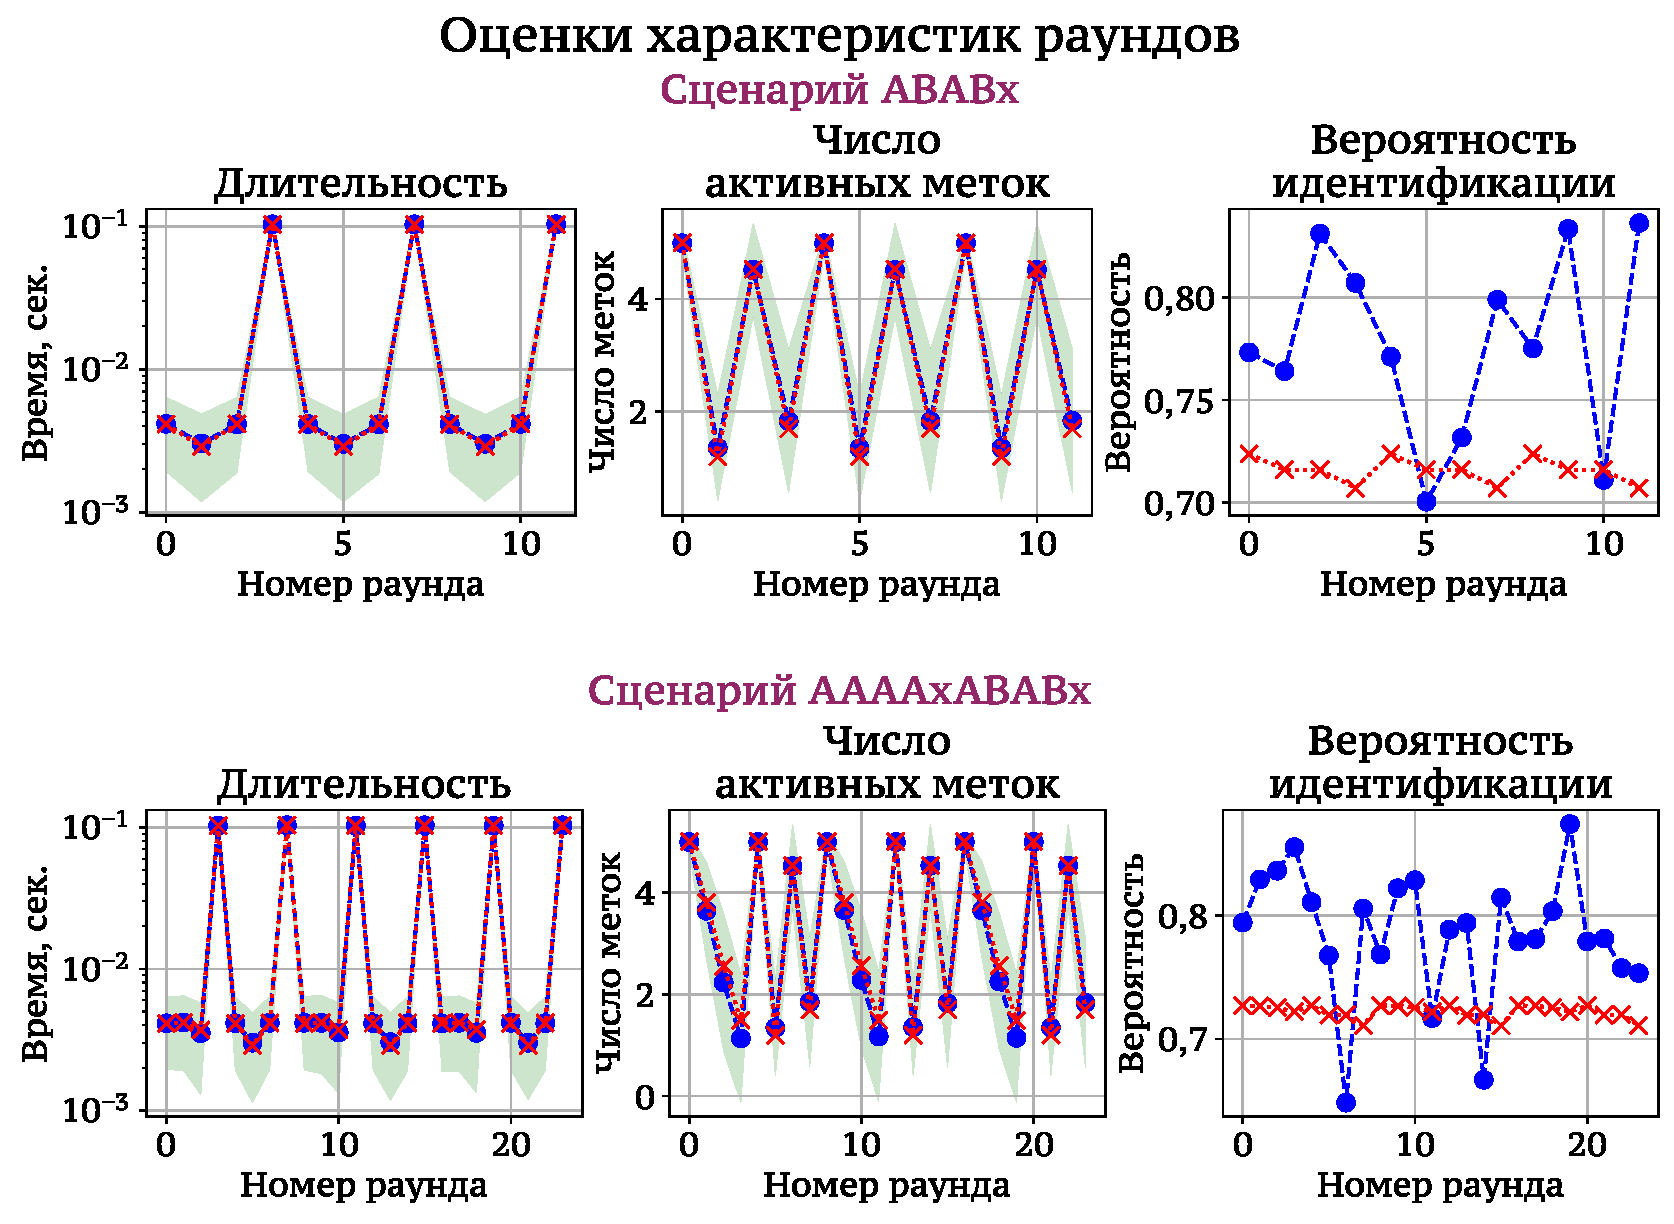
\includegraphics[width=0.8\textwidth]{chapter3/ch3_results_rounds_props}
  }
  \caption{Оценки характеристик раундов.}
  \label{fig:ch3_results_rounds_props}
\end{figure}

Результаты сравнения оценок длительностей раундов, среднего числа активных меток и вероятностей идентификации (при поступлении в заданном раунде), полученных с помощью аналитической и имитационной модели для смешанных сценариев, приведены на рис.~\ref{fig:ch3_results_rounds_props}. При построении результатов использовался множитель раундов при свертке $K_c = 3$. Можно видеть, что оценки длительности и среднего числа аквтиных меток практически полностью совпадают (серая область "--- разброс оценок из имитационной модели). В то же время, оценки вероятности идентификации отличаются, хотя и незначительно.

Из полученных результатов можно сделать вывод, что фоновый процесс позволяет очень точно оценить длительность раундов и среднее число активных меток. Оценки вероятности идентификации, полученные с помощью аналитики, оказываются немного ниже, чем оценки, полученные из имитационной модели.




\subsection{Расчет вероятности идентификации}

Для каждого сценария были рассчитаны вероятности идентификации с помощью аналитической и имитационной моделей. Результаты сравнения приведены на рис.~\ref{fig:ch3_results_prob_cmp}. Рассматривались три различных интервала между поступлениями меток: очень короткий (0,2~сек), средний (0,4~сек) и длинный (1~сек). Так как время нахождения каждой метки в области чтения $T_L = 2,5$~сек фиксировано, то этим значениям соответствуют различные максимальные числа меток в области чтения $\overline{N}$, равные 13, 7 и 3 соответственно. За счет этого можно эффективно учесть влияние коллизий на вероятность идентификации (параметр Q был выбран равным 2, то есть в каждом раунде 4 слота).

\begin{figure}[htb]
	\centerfloat{
    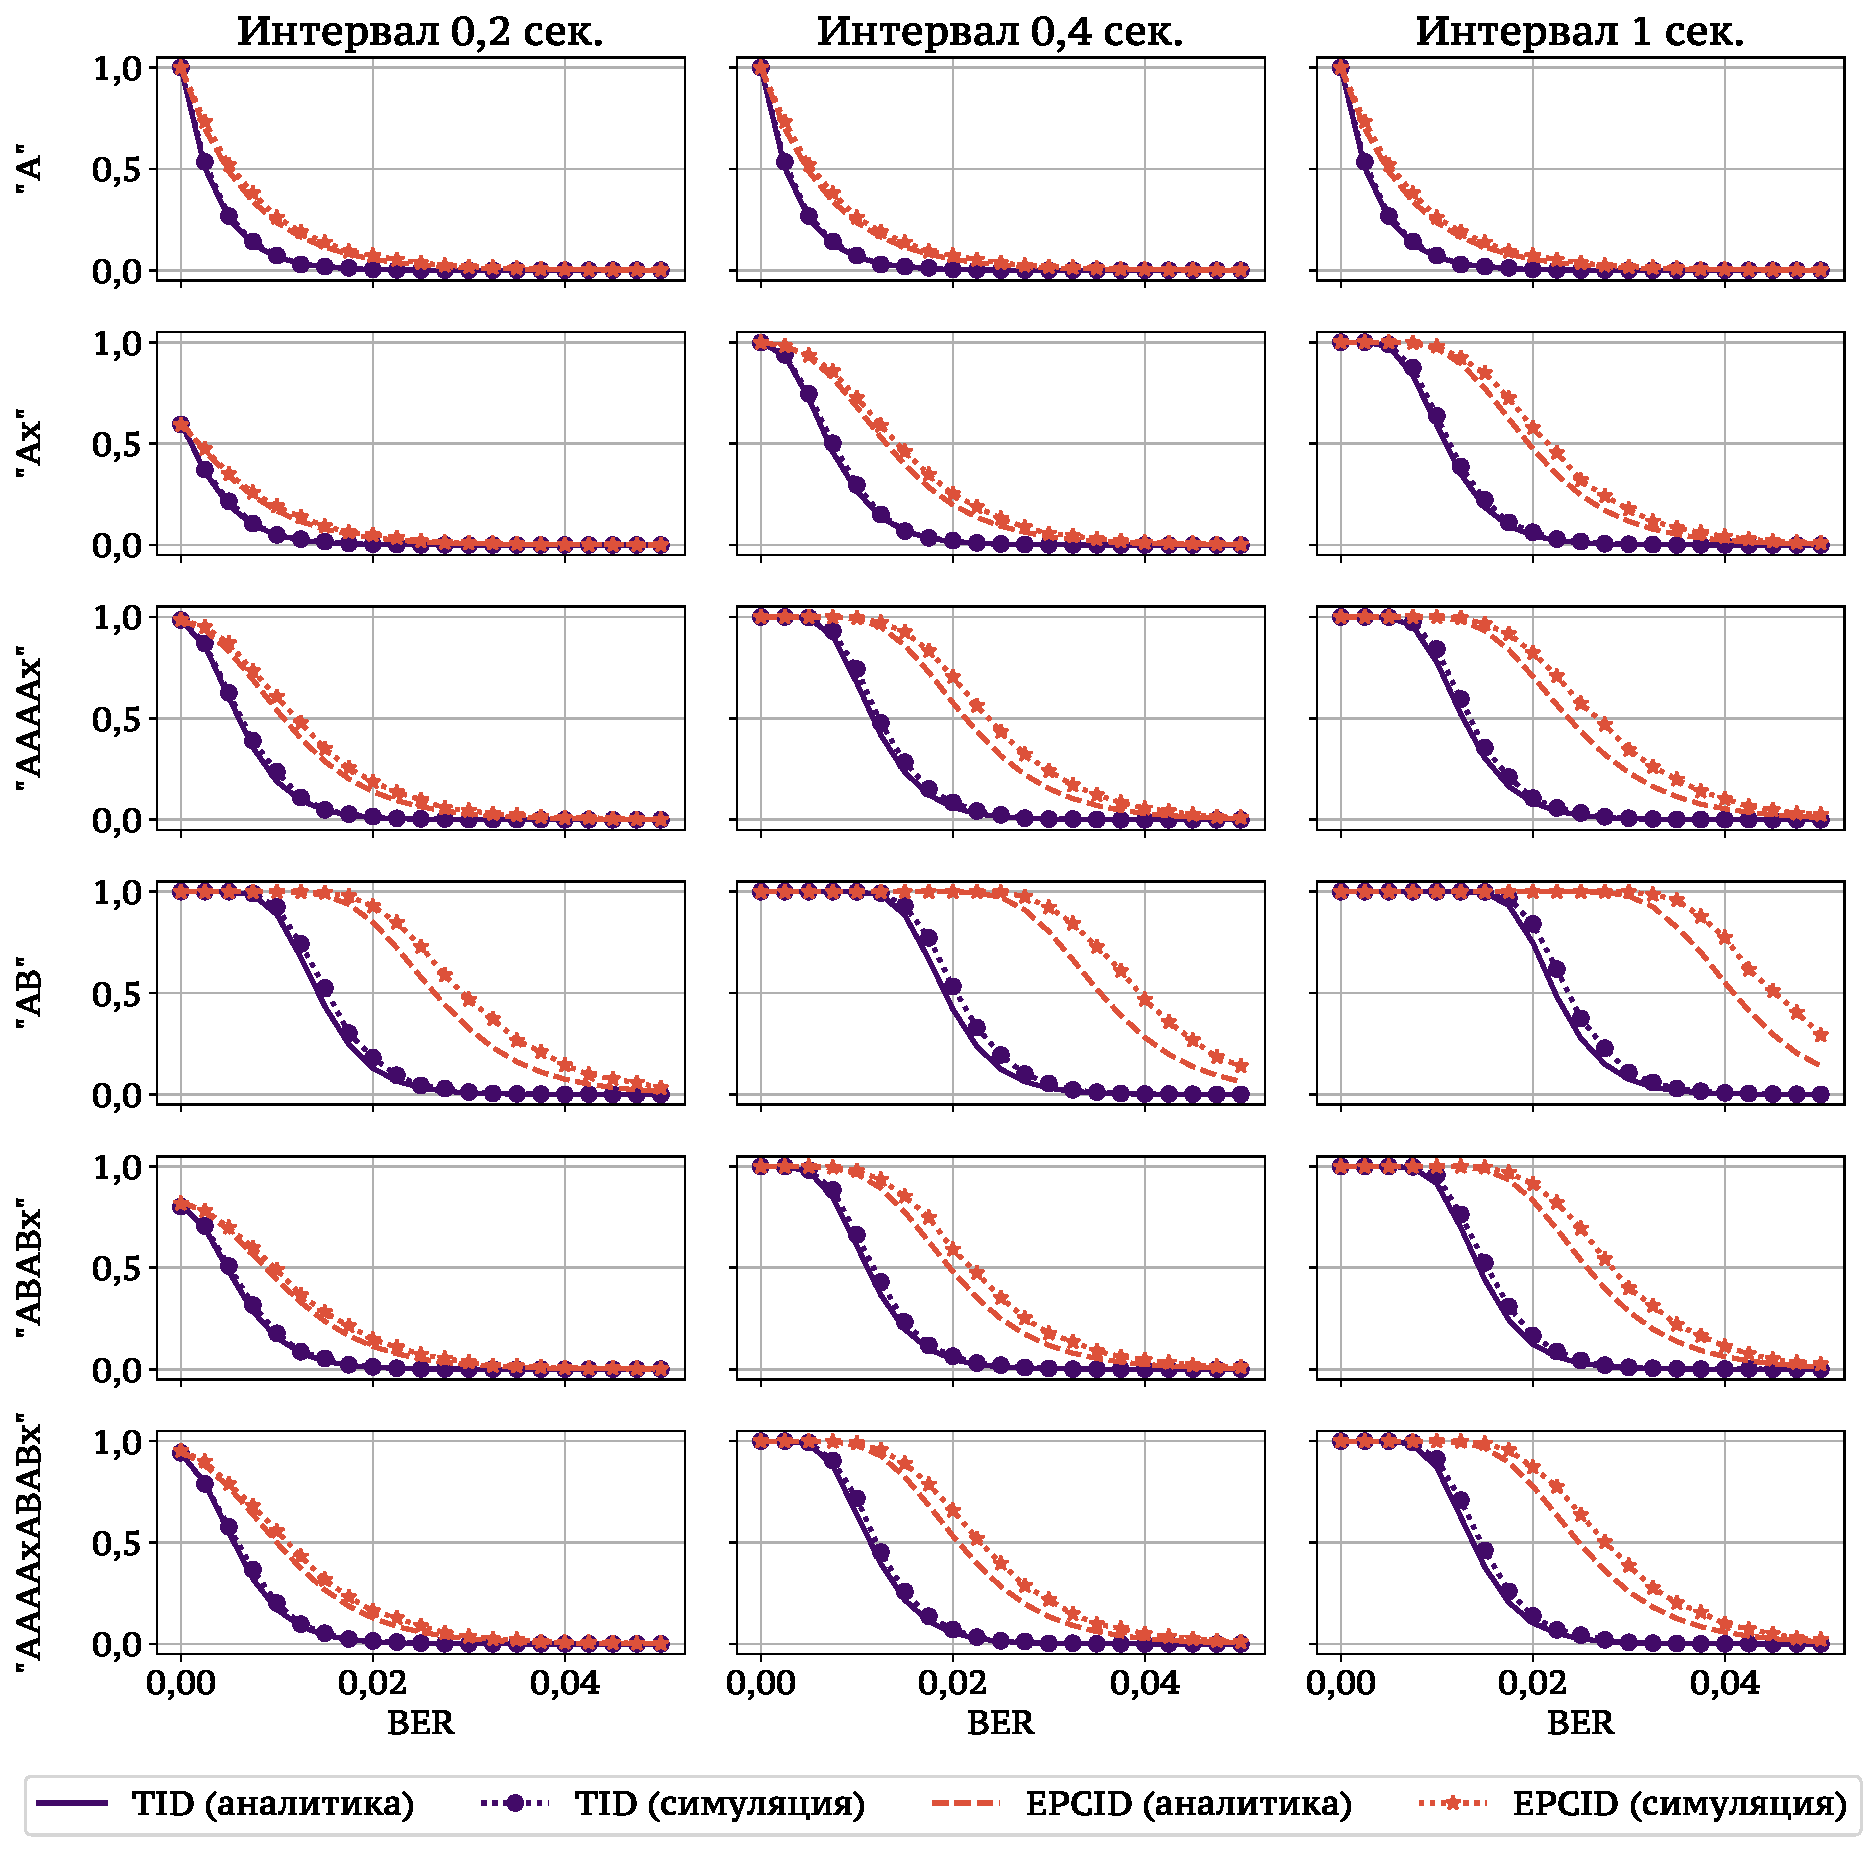
\includegraphics[width=0.9\textwidth]{chapter3/ch3_results_prob_cmp}
  }
  \caption{Сравнение оценок вероятности идентификации, полученных с помощью аналитической и имитационной модели.}
  \label{fig:ch3_results_prob_cmp}
\end{figure}

Результаты, приведенные на рис.~\ref{fig:ch3_results_prob_cmp}, показывают, что оценки оказываются во всех случаях близки, характеры зависимостей от BER совпадают, но оценки аналитической модели всегда несколько ниже. Отметим, что на практике при BER > 0,02 вероятность успешно передать данные слишком мала, поэтому основной интерес представляют левые половины графиков, а на них отклонение оказывается совсем малым. Таким образом, при небольших значениях BER аналитическая модель позволяет достаточно точно оценить вероятность идентификации.

\begin{figure}[htb]
	\centerfloat{
    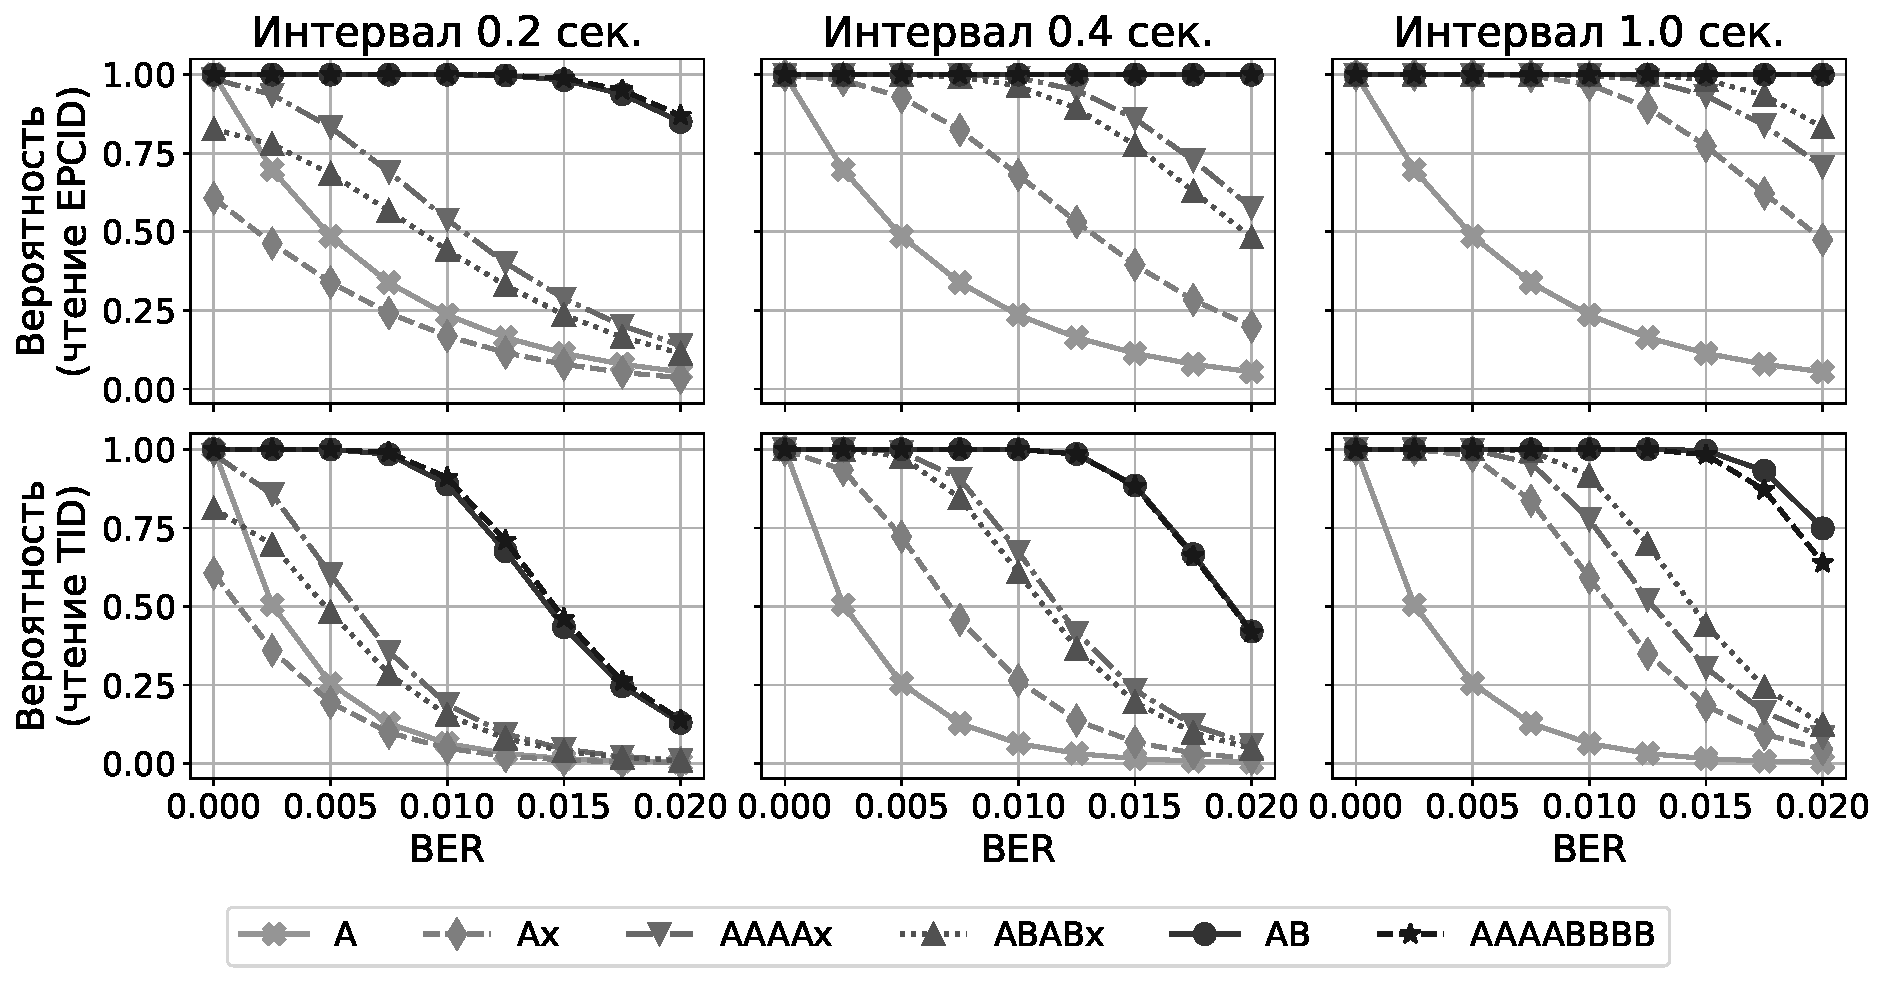
\includegraphics[width=0.9\textwidth]{chapter3/ch3_results_probs}
  }
  \caption{Вероятности идентификации в различных сценариях.}
  \label{fig:ch3_results_probs}
\end{figure}

Чтобы более наглядно оценить влияние выбора сценария на вероятность идентификации, на рис.~\ref{fig:ch3_results_probs} показаны оценки, полученные с помощью аналитической модели для различных сценариев и интервалов. Самыми неэффективными оказываются сценарий $A^0$ (без сбросов питания и смены флагов) и $A^1$ (сброс питания после каждого раунда), причем первый из них дает практически идентичные результаты независимо от интервала, а второй оказывается тем менее эффективен, чем короче интервал. Низкую эффективность сценария $A^0$ и слабую зависимость от длины интервалов между поступлениями можно объяснить тем, что после первой ошибки в передаче EPCID метка инвертирует флаг и больше не участвует в опросе. Так как новая метка успевает ошибиться (или успешно передать идентификатор) в течение первых раундов после поступления, к моменту появления следующей метки она уже неактивна, поэтому не влияет на коллизии. В сценарии $A^1$, напротив, в каждом раунде участвуют все метки, находящиеся в области чтения, поэтому при большом числе меток вероятность идентификации снижается из-за коллизий. Кроме того, на частые сбросы питания расходуется очень много времени, из-за чего вероятность снижается и при небольшом числе меток. Примечательно, что при самых коротких интервалах вероятность идентификации в сценарии $A^1$ оказывается даже ниже, чем в сценарии $A^0$.

Самые лучшие результаты показывают сценарии, в которых не используется сброс питания, а только периодические смены флагов. При этом, чем больше меток в области чтения, тем реже стоит делать переключения, и наоборот: при идентификации по TID и поступлении меток каждый 0,2~сек вероятность идентификации в сценарии $A^0A^0A^0A^0B^0B^0B^0B^0$ оказывается немного выше, чем в сценарии $A^0B^0$, а при интервале 1~сек "--- наоборот. Этот эффект можно объяснить тем, что более редкие переключения позволяют более эффективно противостоять росту вероятности коллизии при увеличении числа меток в области чтения. Отметим, что при значениях BER до 0,01 различий практически нет.

Сценарии со сбросами питания дают вероятность идентификации существенно ниже, чем сценарии со сменой флага и без сброса питания. Примечательно, что при коротких интервалах выгоднее не менять флаг (сценарий $A^0A^0A^0A^1$), чем изменять его в дополнение к сбросу питания (сценарий $A^0B^0A^0B^1$). Как и для сценариев со сменой флага без сброса питания, это можно объяснить тем, что смены флагов ведут к увеличению вероятности коллизии.

В целом, можно сделать вывод о том, что сбросов питания лучше избегать, если есть возможность периодически изменять флаги опроса. Если по какой-то причине возможности менять флаги нет, то желательно периодически сбрасывать питание во всех случаях, кроме присутствия большого числа меток. Отметим, что часто сбросы питания возникают независимо, из-за смены антенн или необходимости периодических отключений по требованиям регулирующих органов.


\subsection{Исследование ошибок в оценке вероятности идентификации}

Полагая результаты имитационного моделирования точными, вычислим относительную и абсолютную ошибки в определении вероятности идентификации. На рис.~\ref{fig:ch3_results_rel_errors} в левой части показаны относительные ошибки для сценариев, в которых происходит только отключение питания, только смена флагов или и то, и другое (либо ни то, ни другое). Ошибки показаны с помощью свечного графика (график типа ящик с усами), на котором тело свечи ограничено первым и третьим квартилем, горизонтальная линия в свече показывает медиану, а границы усов взяты по 1-му и 99-му проценталям.

\begin{figure}[htb]
	\centerfloat{
    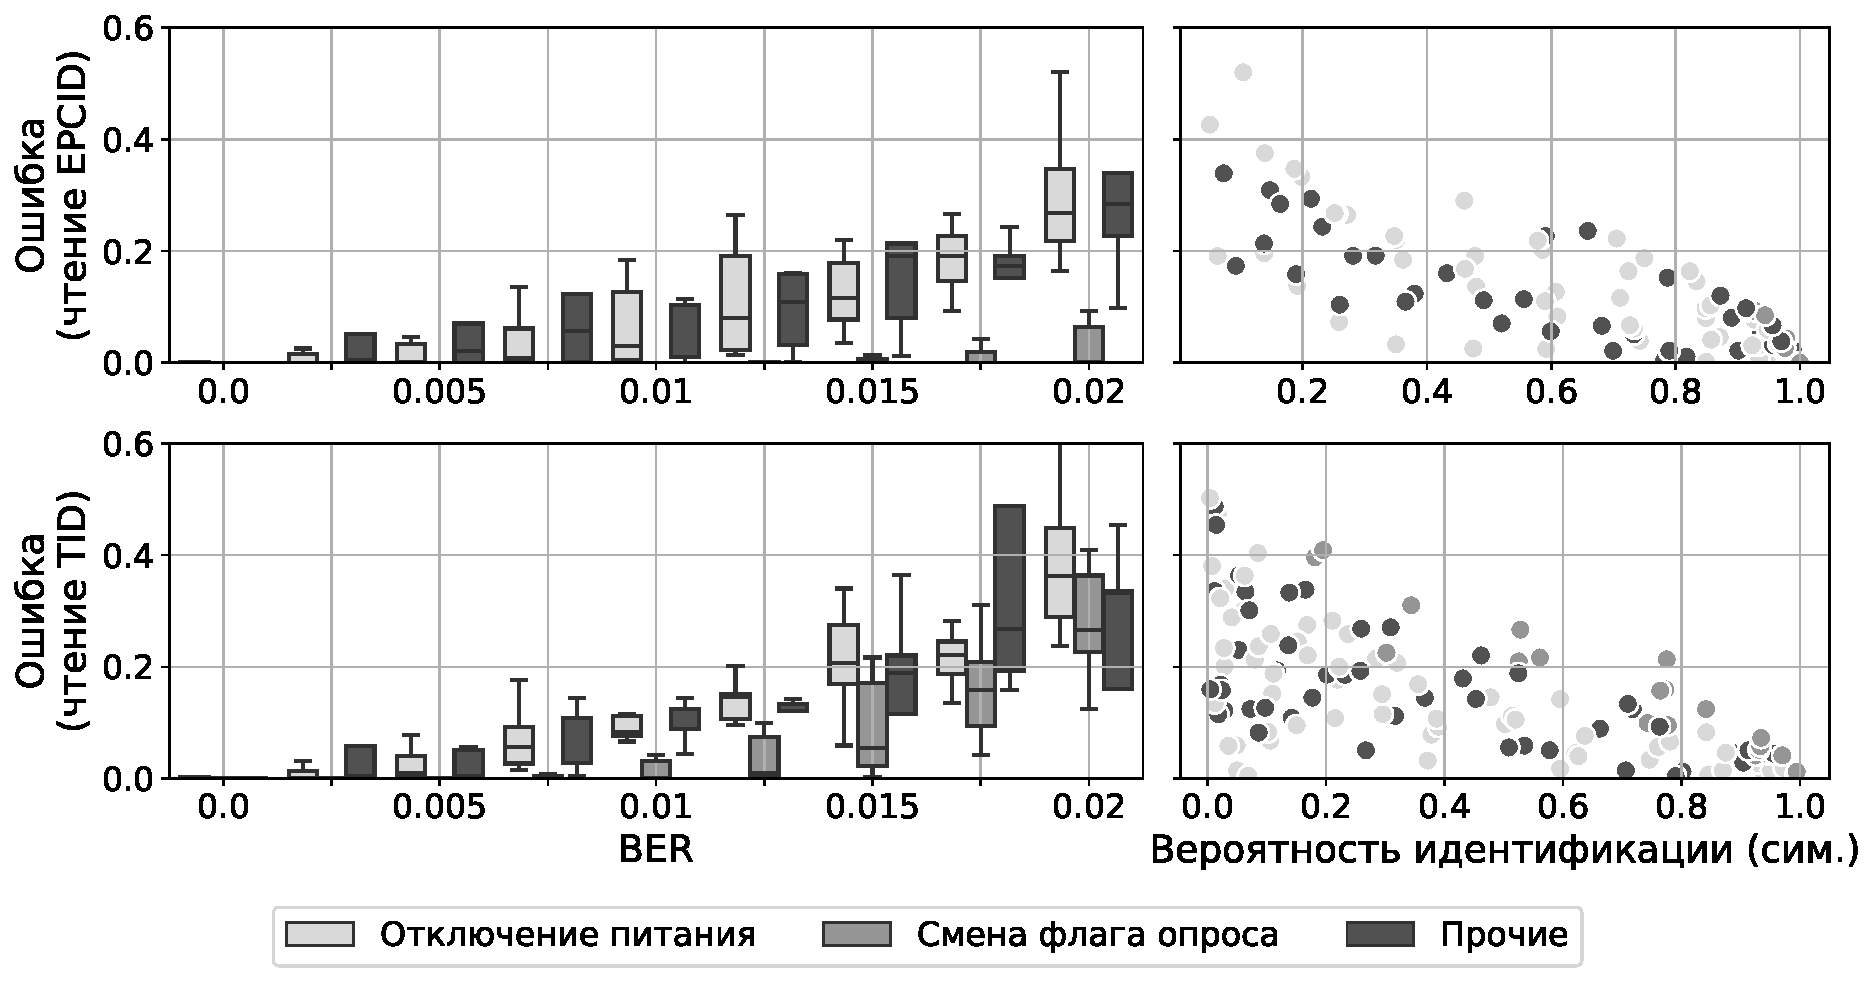
\includegraphics[width=0.9\textwidth]{chapter3/ch3_results_rel_errors}
  }
  \caption{Относительные ошибки оценки вероятности идентификации.}
  \label{fig:ch3_results_rel_errors}
\end{figure}

Чтобы лучше понять причины этого роста, на правой части графика изображена диаграмма рассеяния, точки которой соответствуют ошибкам, полученным для тех входных данных, на которых была вычислена вероятность идентификации, отмеченная на абсциссе. Из этих диаграмм можно видеть, что относительные ошибки увеличиваются при уменьшении вероятности идентификации, что может говорить о небольшой абсолютной ошибке, которая не уменьшается до нуля при уменьшении вероятности идентификации. Чтобы подтвердить это предположение, на рис.~\ref{fig:ch3_results_abs_errors} показаны абсолютные ошибки. Можно видеть, что для большей части сценариев медианы ошибок не превосходят 0,05, и только при достаточно большом BER в некоторых сценариях приближаются к 0,1. Так как при росте BER вероятность идентификации уменьшается, то, соответственно, растет и относительная ошибка.


\begin{figure}[htb]
	\centerfloat{
    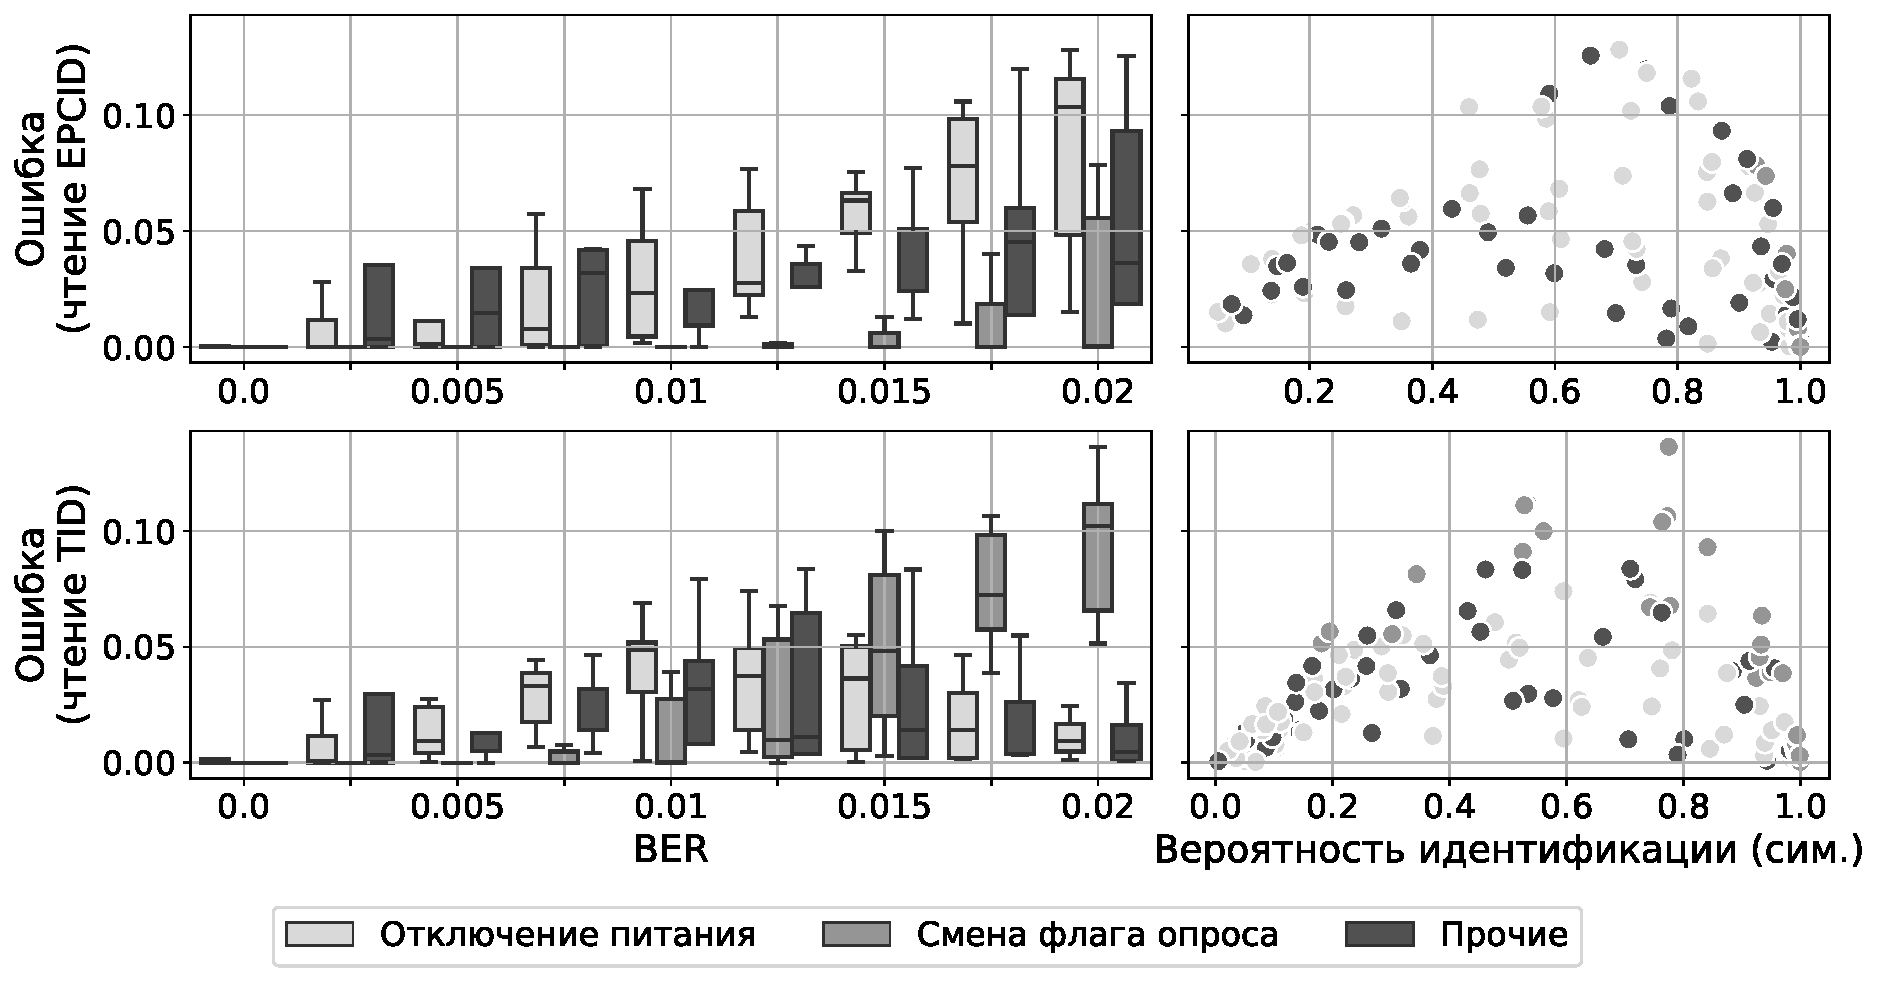
\includegraphics[width=0.9\textwidth]{chapter3/ch3_results_abs_errors}
  }
  \caption{Абсолютные ошибки оценки вероятности идентификации.}
  \label{fig:ch3_results_abs_errors}
\end{figure}

В целом, полученные результаты говорят о том, что точность аналитической модели оказывается достаточно высокой, для низких значениях $\text{BER} < 0,01$ относительная ошибка мала: для идентификации по EPCID медианы не превосходят 5\%, а для идентификации по TID "--- 10\%. Для более высоких значений BER относительная ошибка растет до 0,4, но абсолютная ошибка остается достаточно малой, медианные значения не превышает 0,11.



%%%%%%%%%%%%%%%%%%%%%%%%%%%%%%%%%%%%%%%%%%%%%%%%%%%%%%%%%%%%%%%%%%%%%%%%%%%%%%%%
\section{Заключение}\label{sec:ch3_conclusion}
%%%%%%%%%%%%%%%%%%%%%%%%%%%%%%%%%%%%%%%%%%%%%%%%%%%%%%%%%%%%%%%%%%%%%%%%%%%%%%%%
В главе были представлены следующие результаты.

\begin{enumerate}
\item Предложена новая аналитическая модель системы радиочастотной идентификации мобильных меток, позволяющая учитывать сбросы питания считывателем и смены флагов сессий. Модель позволяет находить оценки длительностей раундов и вероятности идентификации меток. Модель включает в себя два неоднородных марковских процесса, описывающих число участвующих в каждом раунде меток, и состояние отдельной метки, для которой вычисляется вероятность идентификации. Переходы между состояниями процессов происходят в соотвтетствии с действиями считывателя и законом изменения числа меток в области чтения.
\item Приведены численные результаты, показывающие, что периодические смены флагов опросов значительно повышают вероятность идентификации движущейся метки. Сбросы питания также повышают вероятность, но менее эфеективны, чем смены флагов опроса.
\item Приведены результаты сравнения аналитической и имитационной моделей, показывающие, что аналитическая модель позволяет находить оценку вероятности идентификации метки с достаточно высокой точностью.
\end{enumerate}

\clearpage
